\documentclass{article}


\usepackage{graphicx}
\usepackage{url}
\usepackage{hyperref}
\usepackage{amsmath}
\usepackage{amssymb}
\usepackage{tipa}
\usepackage{mathtools}
\usepackage{caption}
\usepackage{dsfont}
\graphicspath{{./}}



\hypersetup{
	colorlinks=true,
	urlcolor=blue
}

\usepackage[margin=0.7in]{geometry}
\linespread{1.25}

\title{\fontfamily{bch}\selectfont\Huge Graph Theory Homework v1}
\author{\Large Petrov Maksim M3100}


\begin{document}
	\fontsize{14pt}{16pt}\selectfont
	\maketitle
	
	\section*{Tools and source files}
	Some problems were solved using \href{https://www.minizinc.org/software.html}{MiniZinc Software}. \href{https://www.minizinc.org/doc-2.7.0/en/index.html}{The MiniZinc Handbook} contains detailed instructions on how to run .mnz models and use .dzn data files. In this homework, some models use an adjacency matrix (g.dzn), other models use a list of edges (edges.dzn), others use a list of edges and the number of vertices (edges and v num.dzn). \\\\
	Some of the calculations were done (and the source code for graphviz was obtained) using console C++ applications built with a help of CMake. As the .exe file is located at {\textless}src folder{\textgreater}/Build/Debug, all input and output .txt files in the code begin with '../../' as it's convenient to work with them in the src folder just in IDE.\\\\
	To visualise the graphs, \url{https://dreampuf.github.io/GraphvizOnline/} was used (all graphs visualized using fdp engine).\\\\
	All source files can be found in \href{https://github.com/fish-from-SanDiego/GraphTheoryHW}{HW github repository}:
	MiniZinc files in 'mnz' folder, 'eu.txt' file for the list of the countries, 'tree', 'G', 'dist' and 'G\textbf{\_}star' for C++, 'tex' for \TeX and, finally, 'graphs' for the graphviz templates of $\mathcal{G}^*$, $\mathcal{G}$ and the tree.
	\newpage
	\section*{Task 1}
	The file 'eu.txt' contains a list of European countries, sorted lexicographically, and their \href{https://en.wikipedia.org/wiki/ISO_3166-1_alpha-2#:~:text=ISO%203166%2D1%20alpha%2D2%20codes%20are%20two%2Dletter,special%20areas%20of%20geographical%20interest.}{alpha-2 codes}. The vertices (countries) were labeled in order in this list and by adding alpha-2 code. $\mathcal{G} = \mathcal{G}^*[V(\mathcal{G}^*)\setminus \{\textmd{GB, IS, IE, CY, MT\}}]$. It's also assumed that Spain does not border the UK via Gibraltar.\\\\
	(a) As the only way to minimize number of intersections in the graphviz fdp graph is manually changing the order of nodes in the code and setting 'pos' attribute (which not always works properly) there is still a small number of redundant intersections.
	\begin{figure}[h]
		\centering
		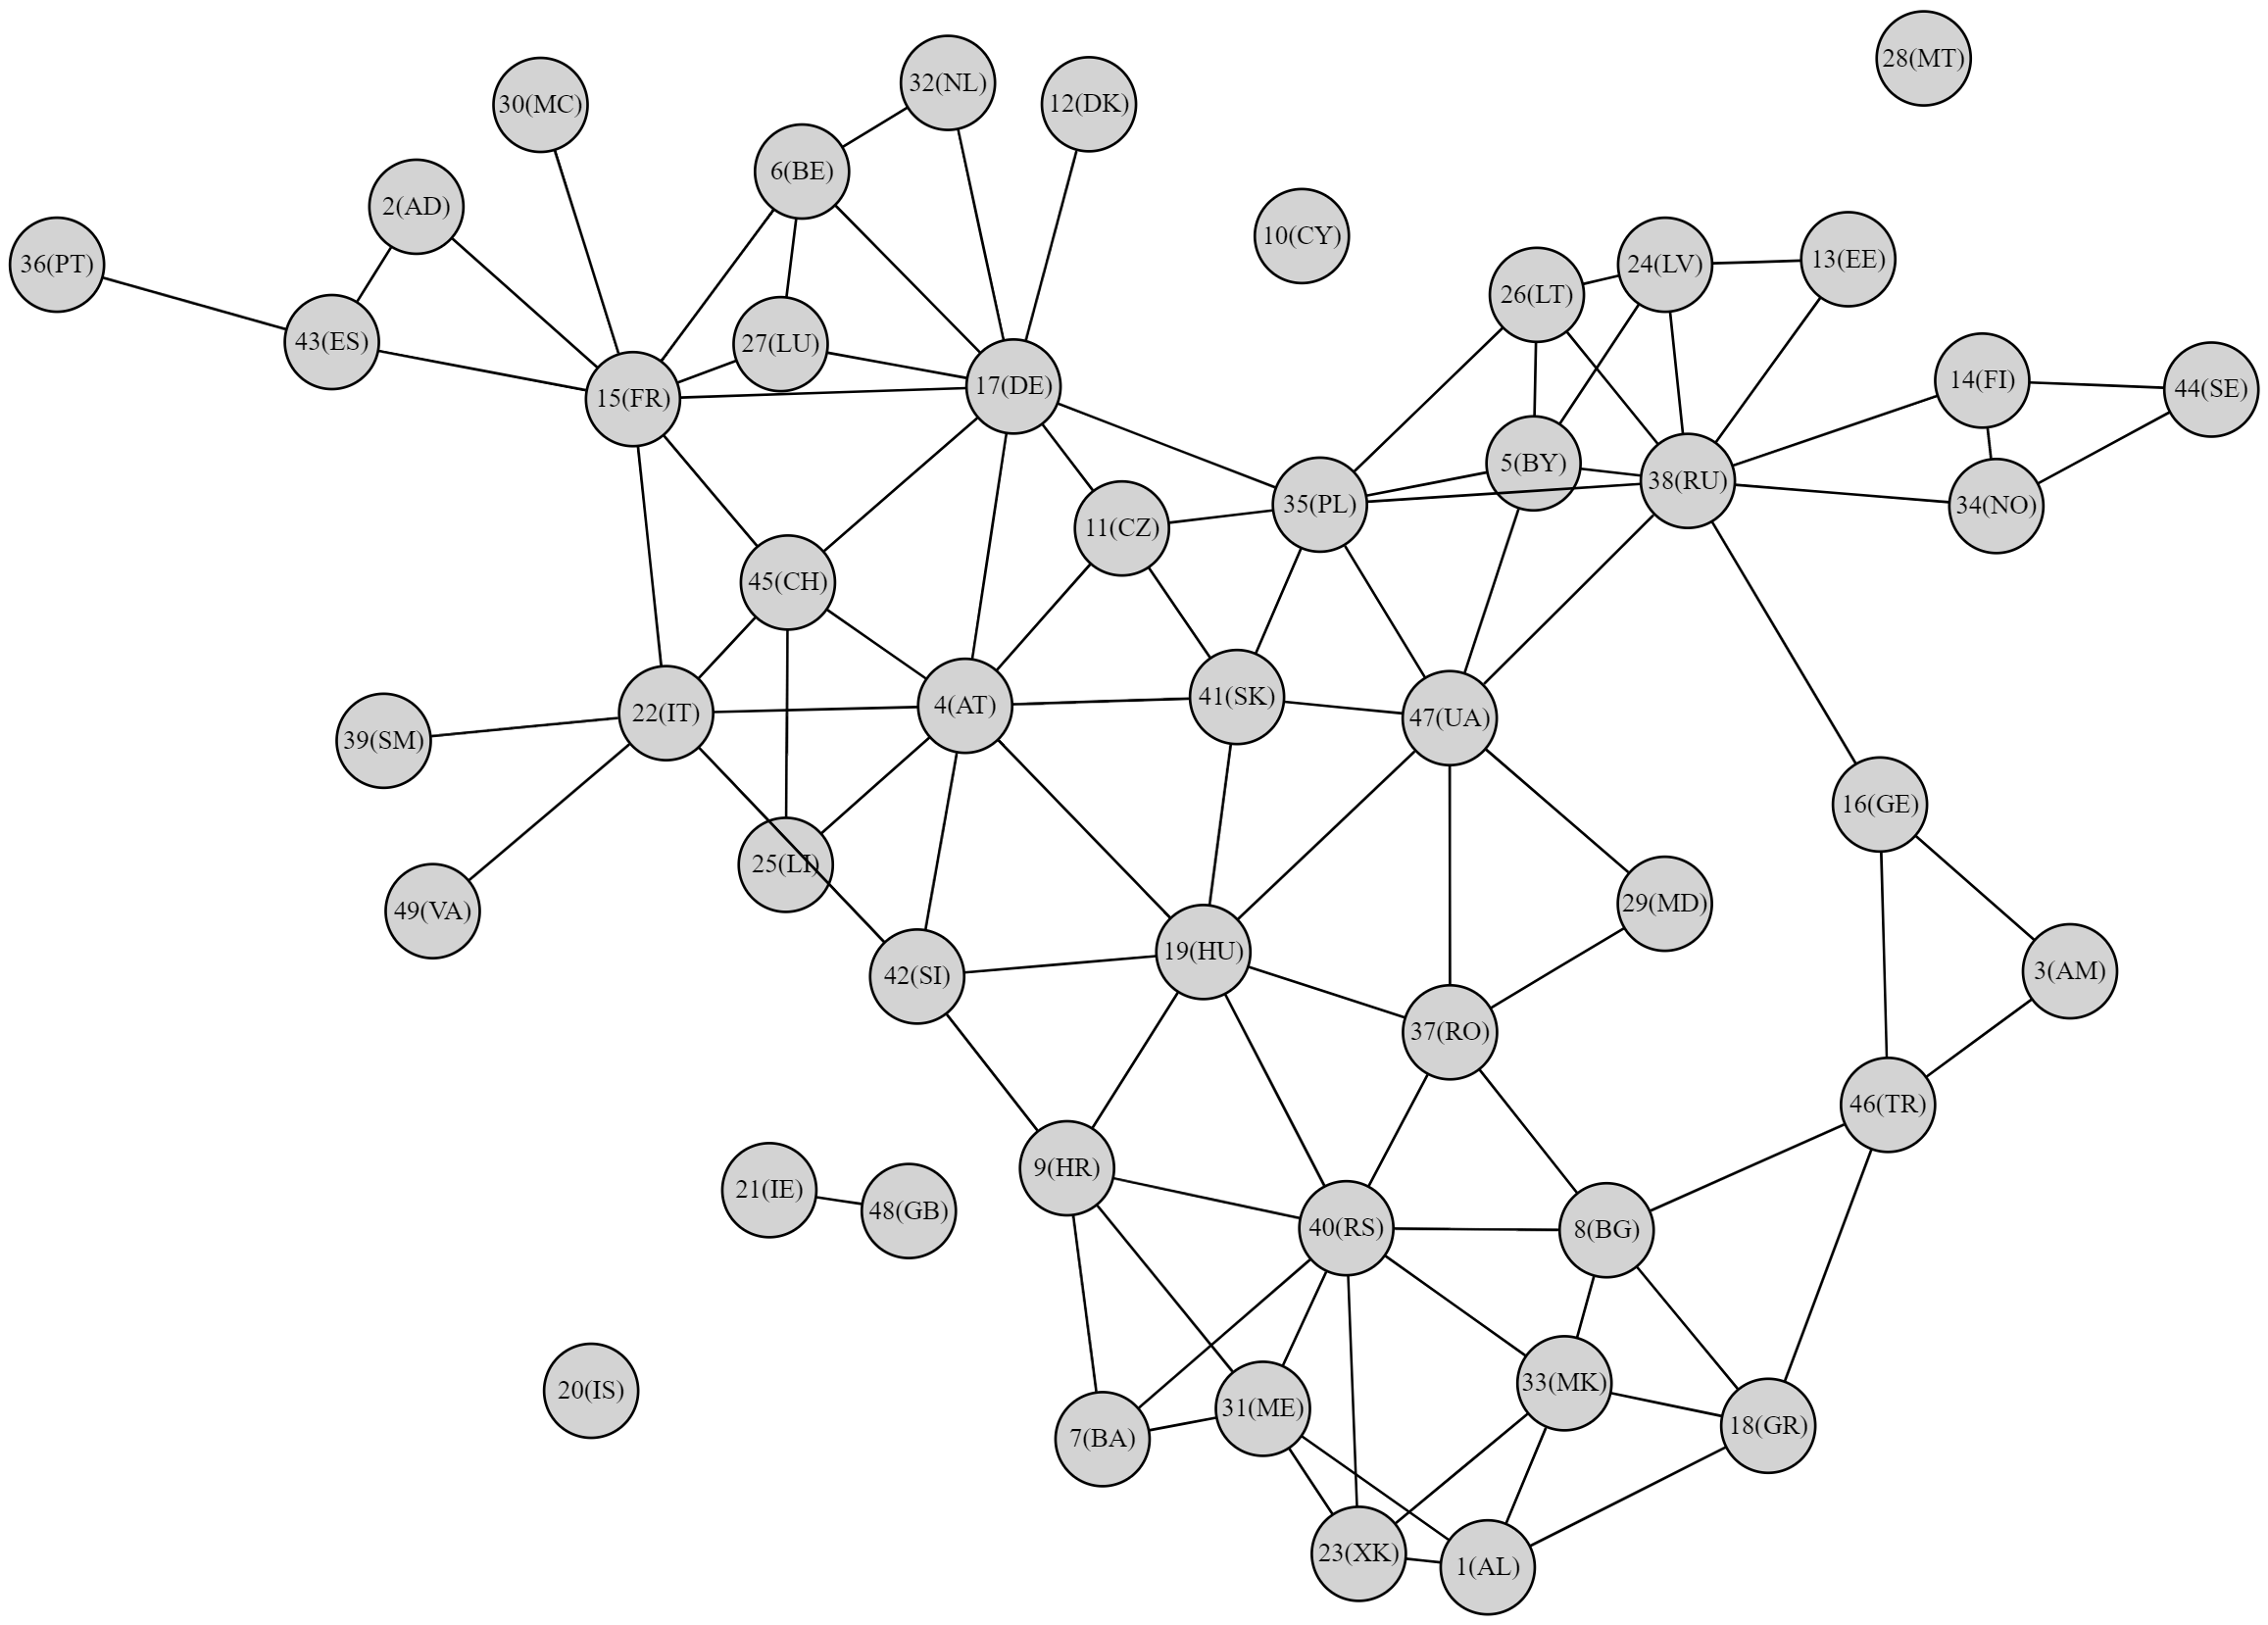
\includegraphics[width=1\textwidth]{G_star.png}
		\caption{$\mathcal{G}^*$ visualization}
	\end{figure}\newpage
	\begin{figure}[h]
		\centering
		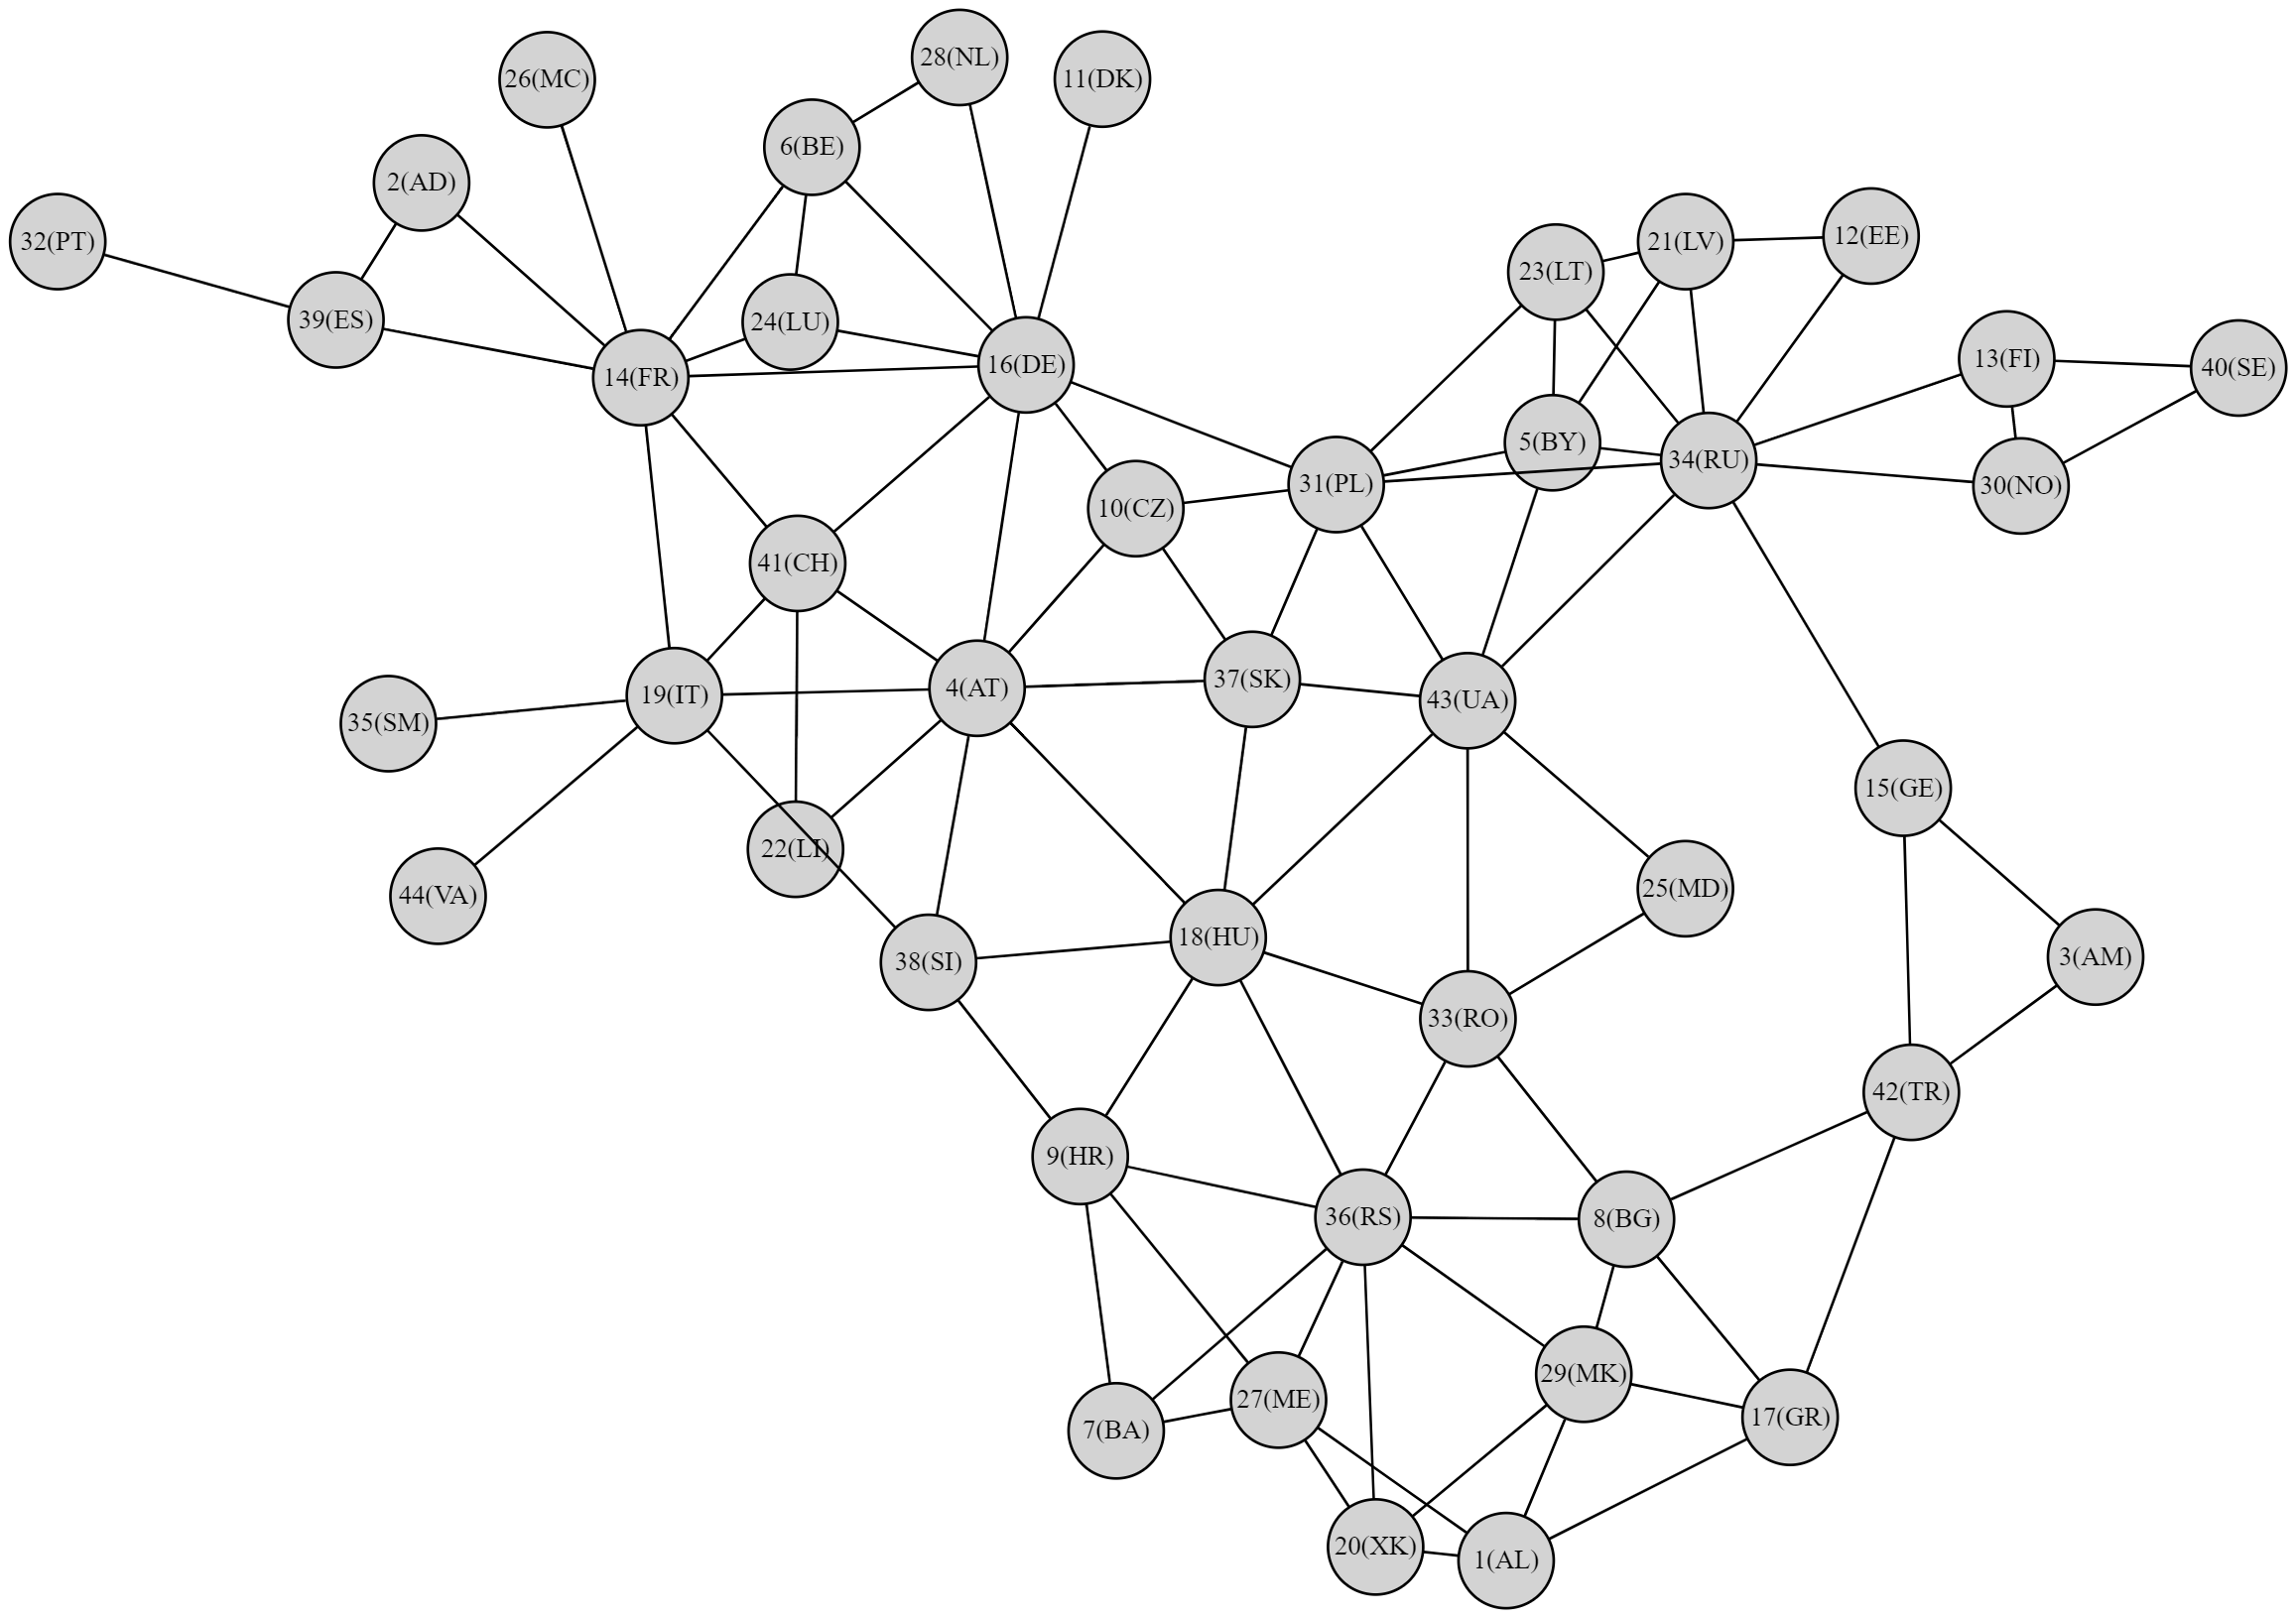
\includegraphics[width=1\textwidth]{G.png}
		\caption{$\mathcal{G}$ visualization}
	\end{figure}\newpage
	(b) Hereinafter vertices of $\mathcal{G}$ have labels different from labels in $\mathcal{G}^*$, so technically it's not subgraph as the labeling function has changed, but it's much more convenient to work with the graph in which vertices are labeled with $1..|V|$ and it's not so difficult to recover original labels as their second parts(alpha-2 codes) haven't changed.
	\\$|V| = 49,~ |E| = 91,~ \delta(\mathcal{G}) = 1$ ($\delta(\mathcal{G}) > 0$ as the graph is connected, e.g. degree of 32(PT) = 1), $\Delta(\mathcal{G}) = 9$ (for 34(RU)), $\textmd{rad}(\mathcal{G}) = 5,~\textmd{diam}(\mathcal{G}) = 8,~\textmd{girth}(\mathcal{G}) = 3,~|\textmd{center}(\mathcal{G})| = 13,~\varkappa(\mathcal{G}) = 1,~\lambda(\mathcal{G}) = 1$. The example of cycle with 3 edges is\\ RS-RO-BG; rad, diam and center are calculated using program from 'dist' folder, it's enough to delete ES or ES-PT to make graph disconnected.
	\begin{figure}[h]
		\centering
		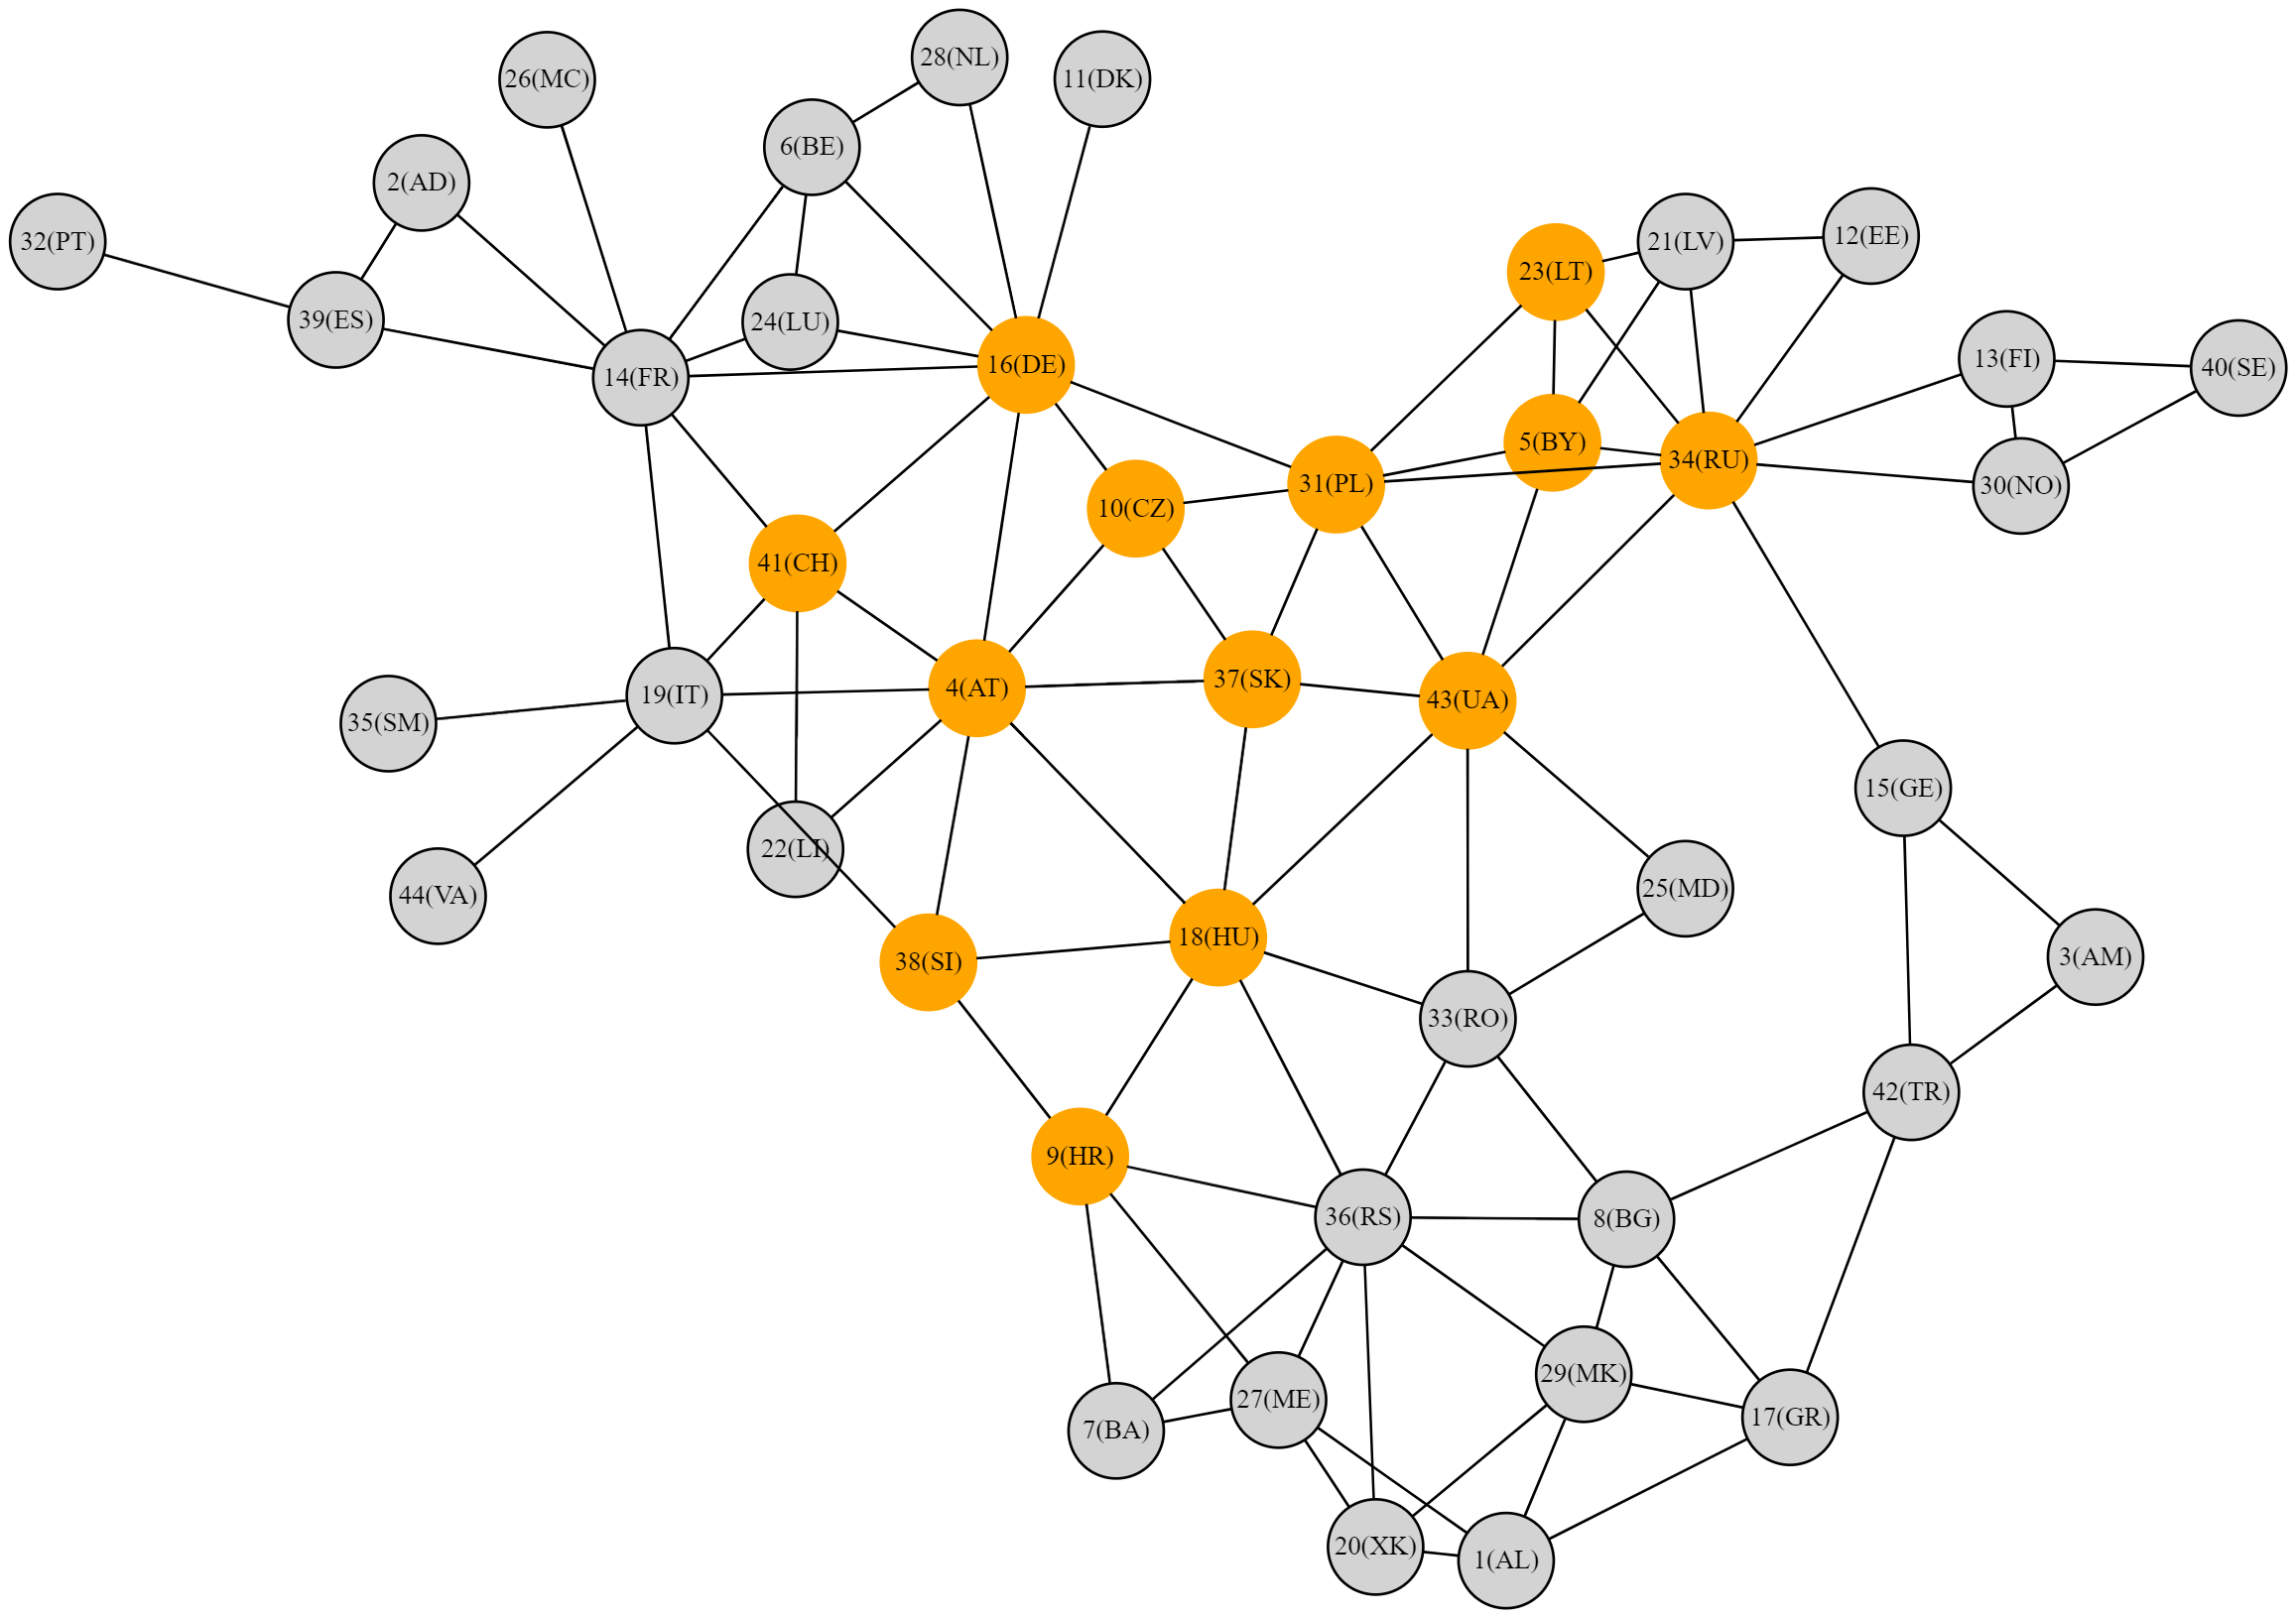
\includegraphics[width=1\textwidth]{center.png}
		\caption{center of $\mathcal{G}$ }
	\end{figure}\newpage
	(c), (d) It's easy to do these using MiniZinc. We just need to check that adjacent vertices (edges) don't have the same color and try to minimize number of colors. Number of vertex colors is 4 and the number of edge colors is 9.
	\begin{figure}[h]
		\centering
		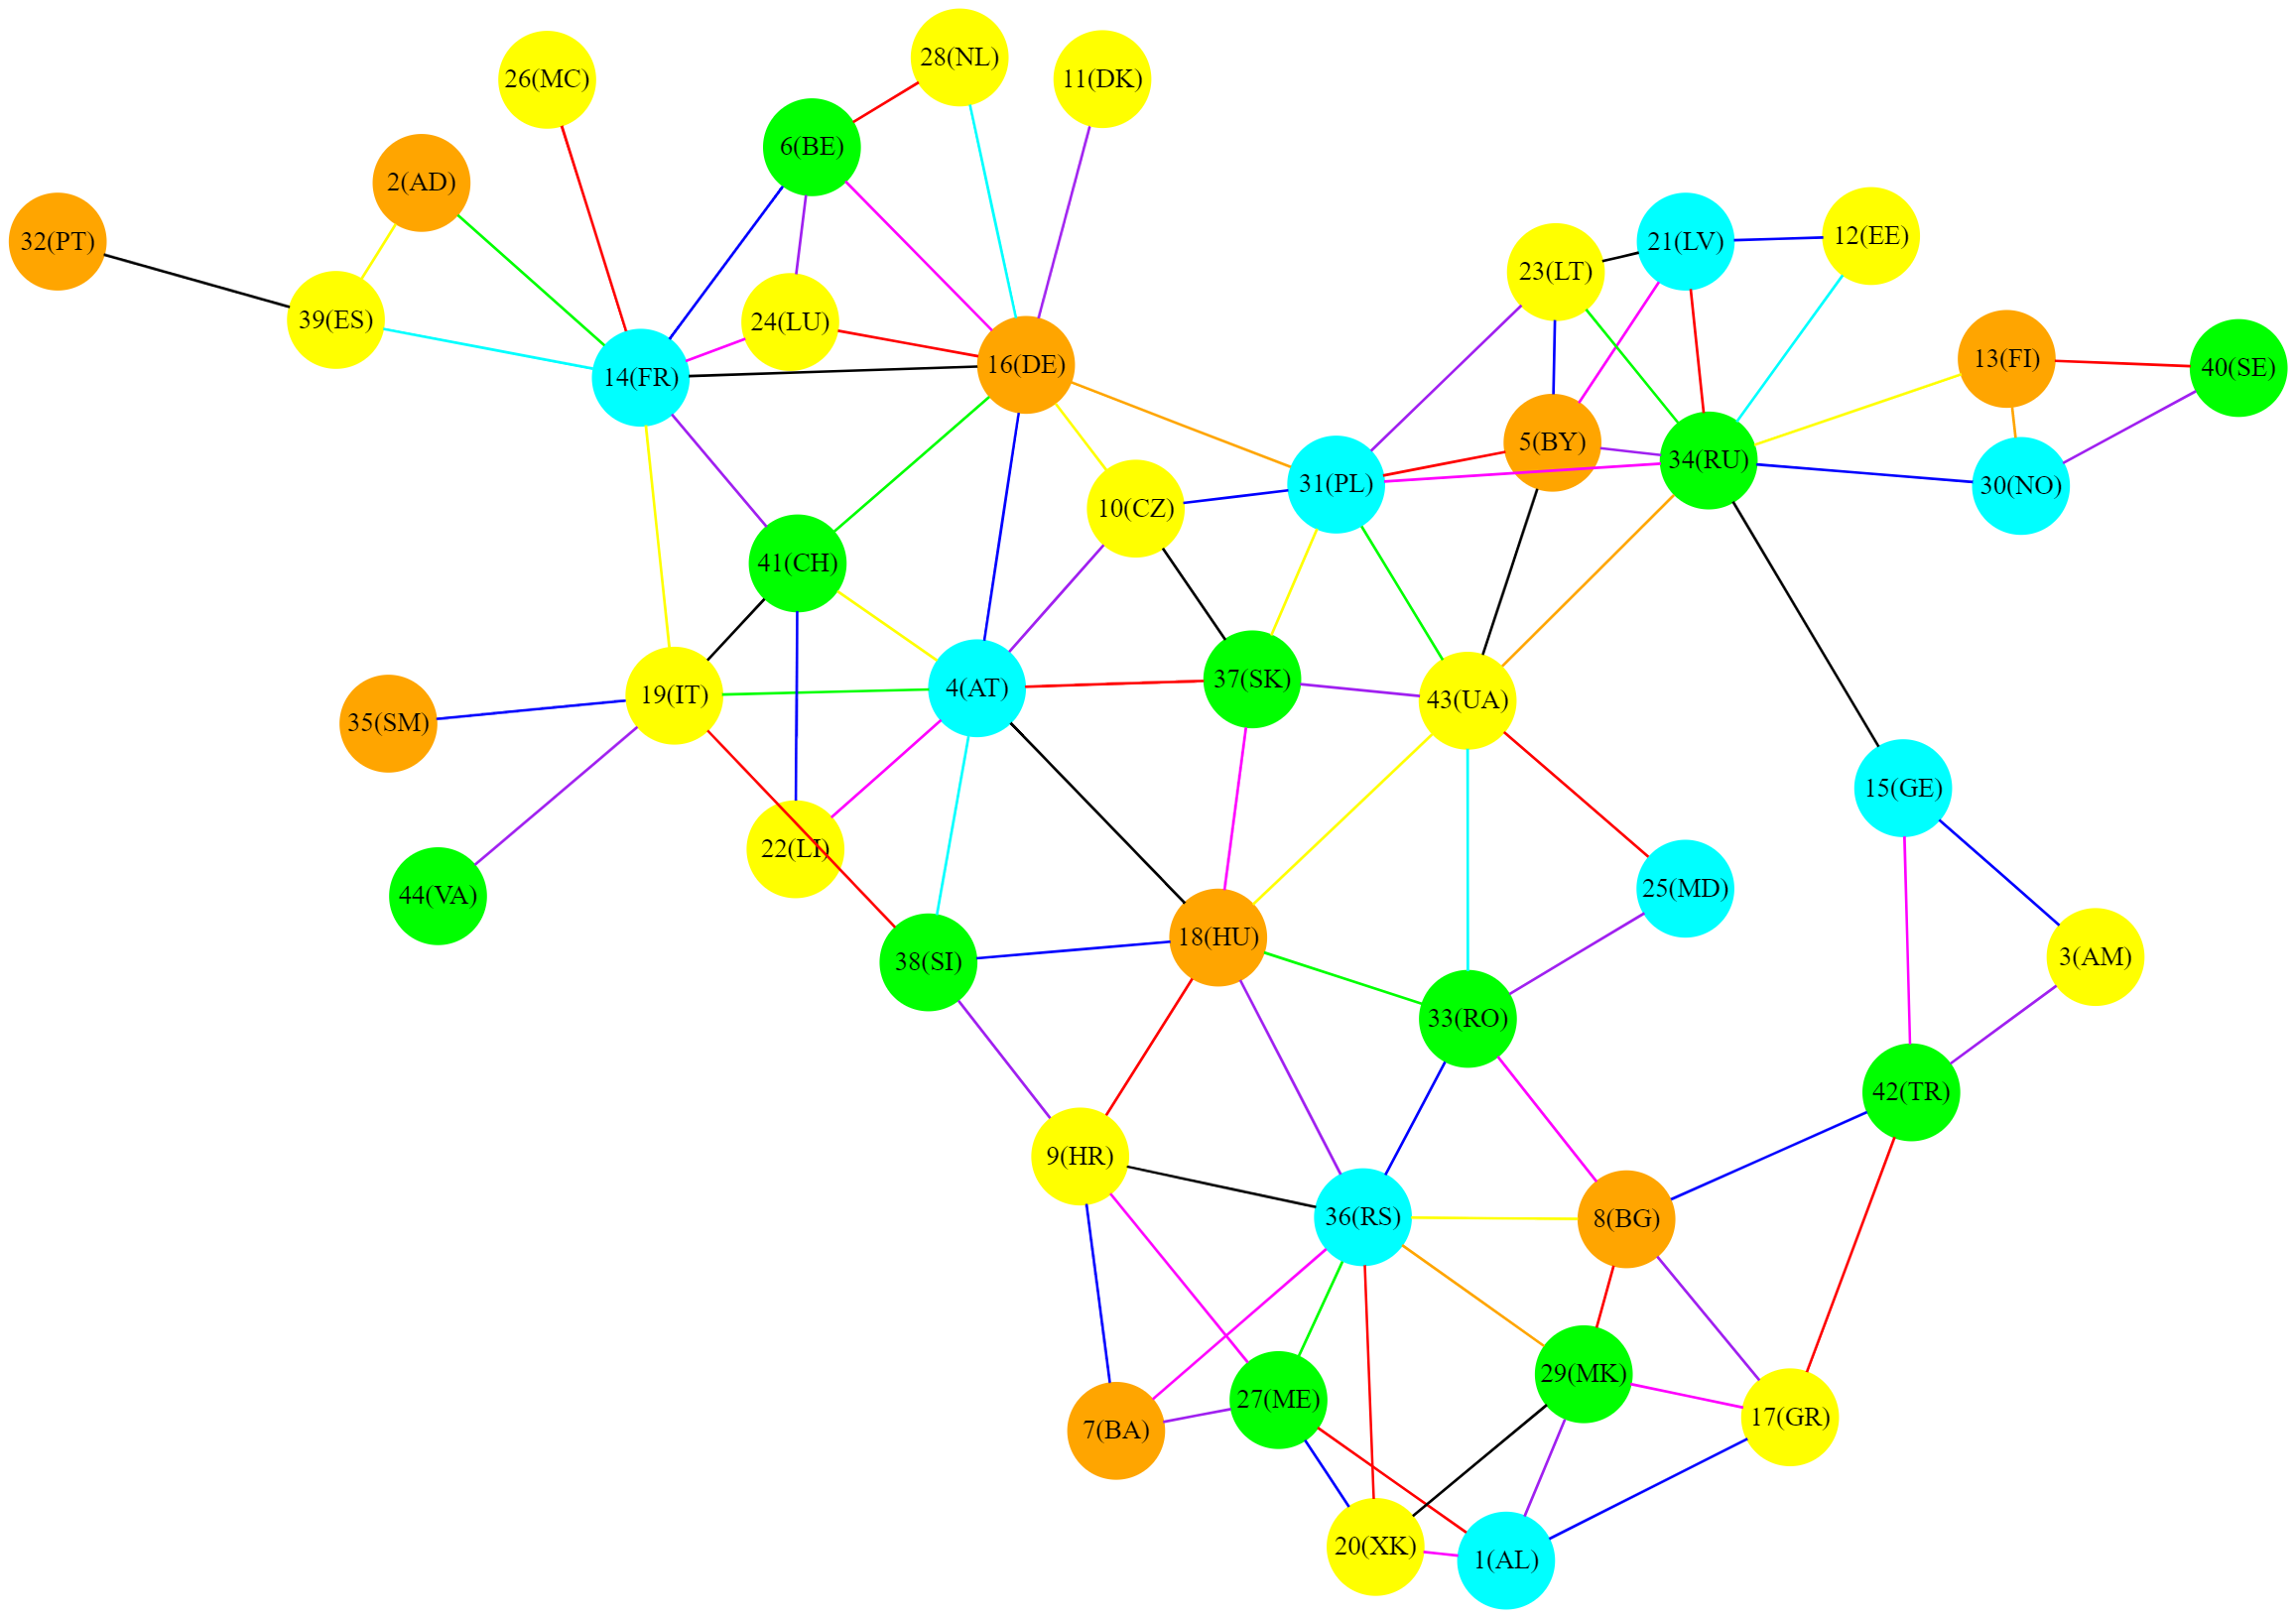
\includegraphics[width=1\textwidth]{v_e_coloring.png}
		\caption{vertex and edge colorings}
	\end{figure}\newpage
	(e) To find the maximum clique via MiniZinc we'll check that every pairwise distinct vertices in clique are adjacent. Size of such clique is 4.
	\begin{figure}[h]
		\centering
		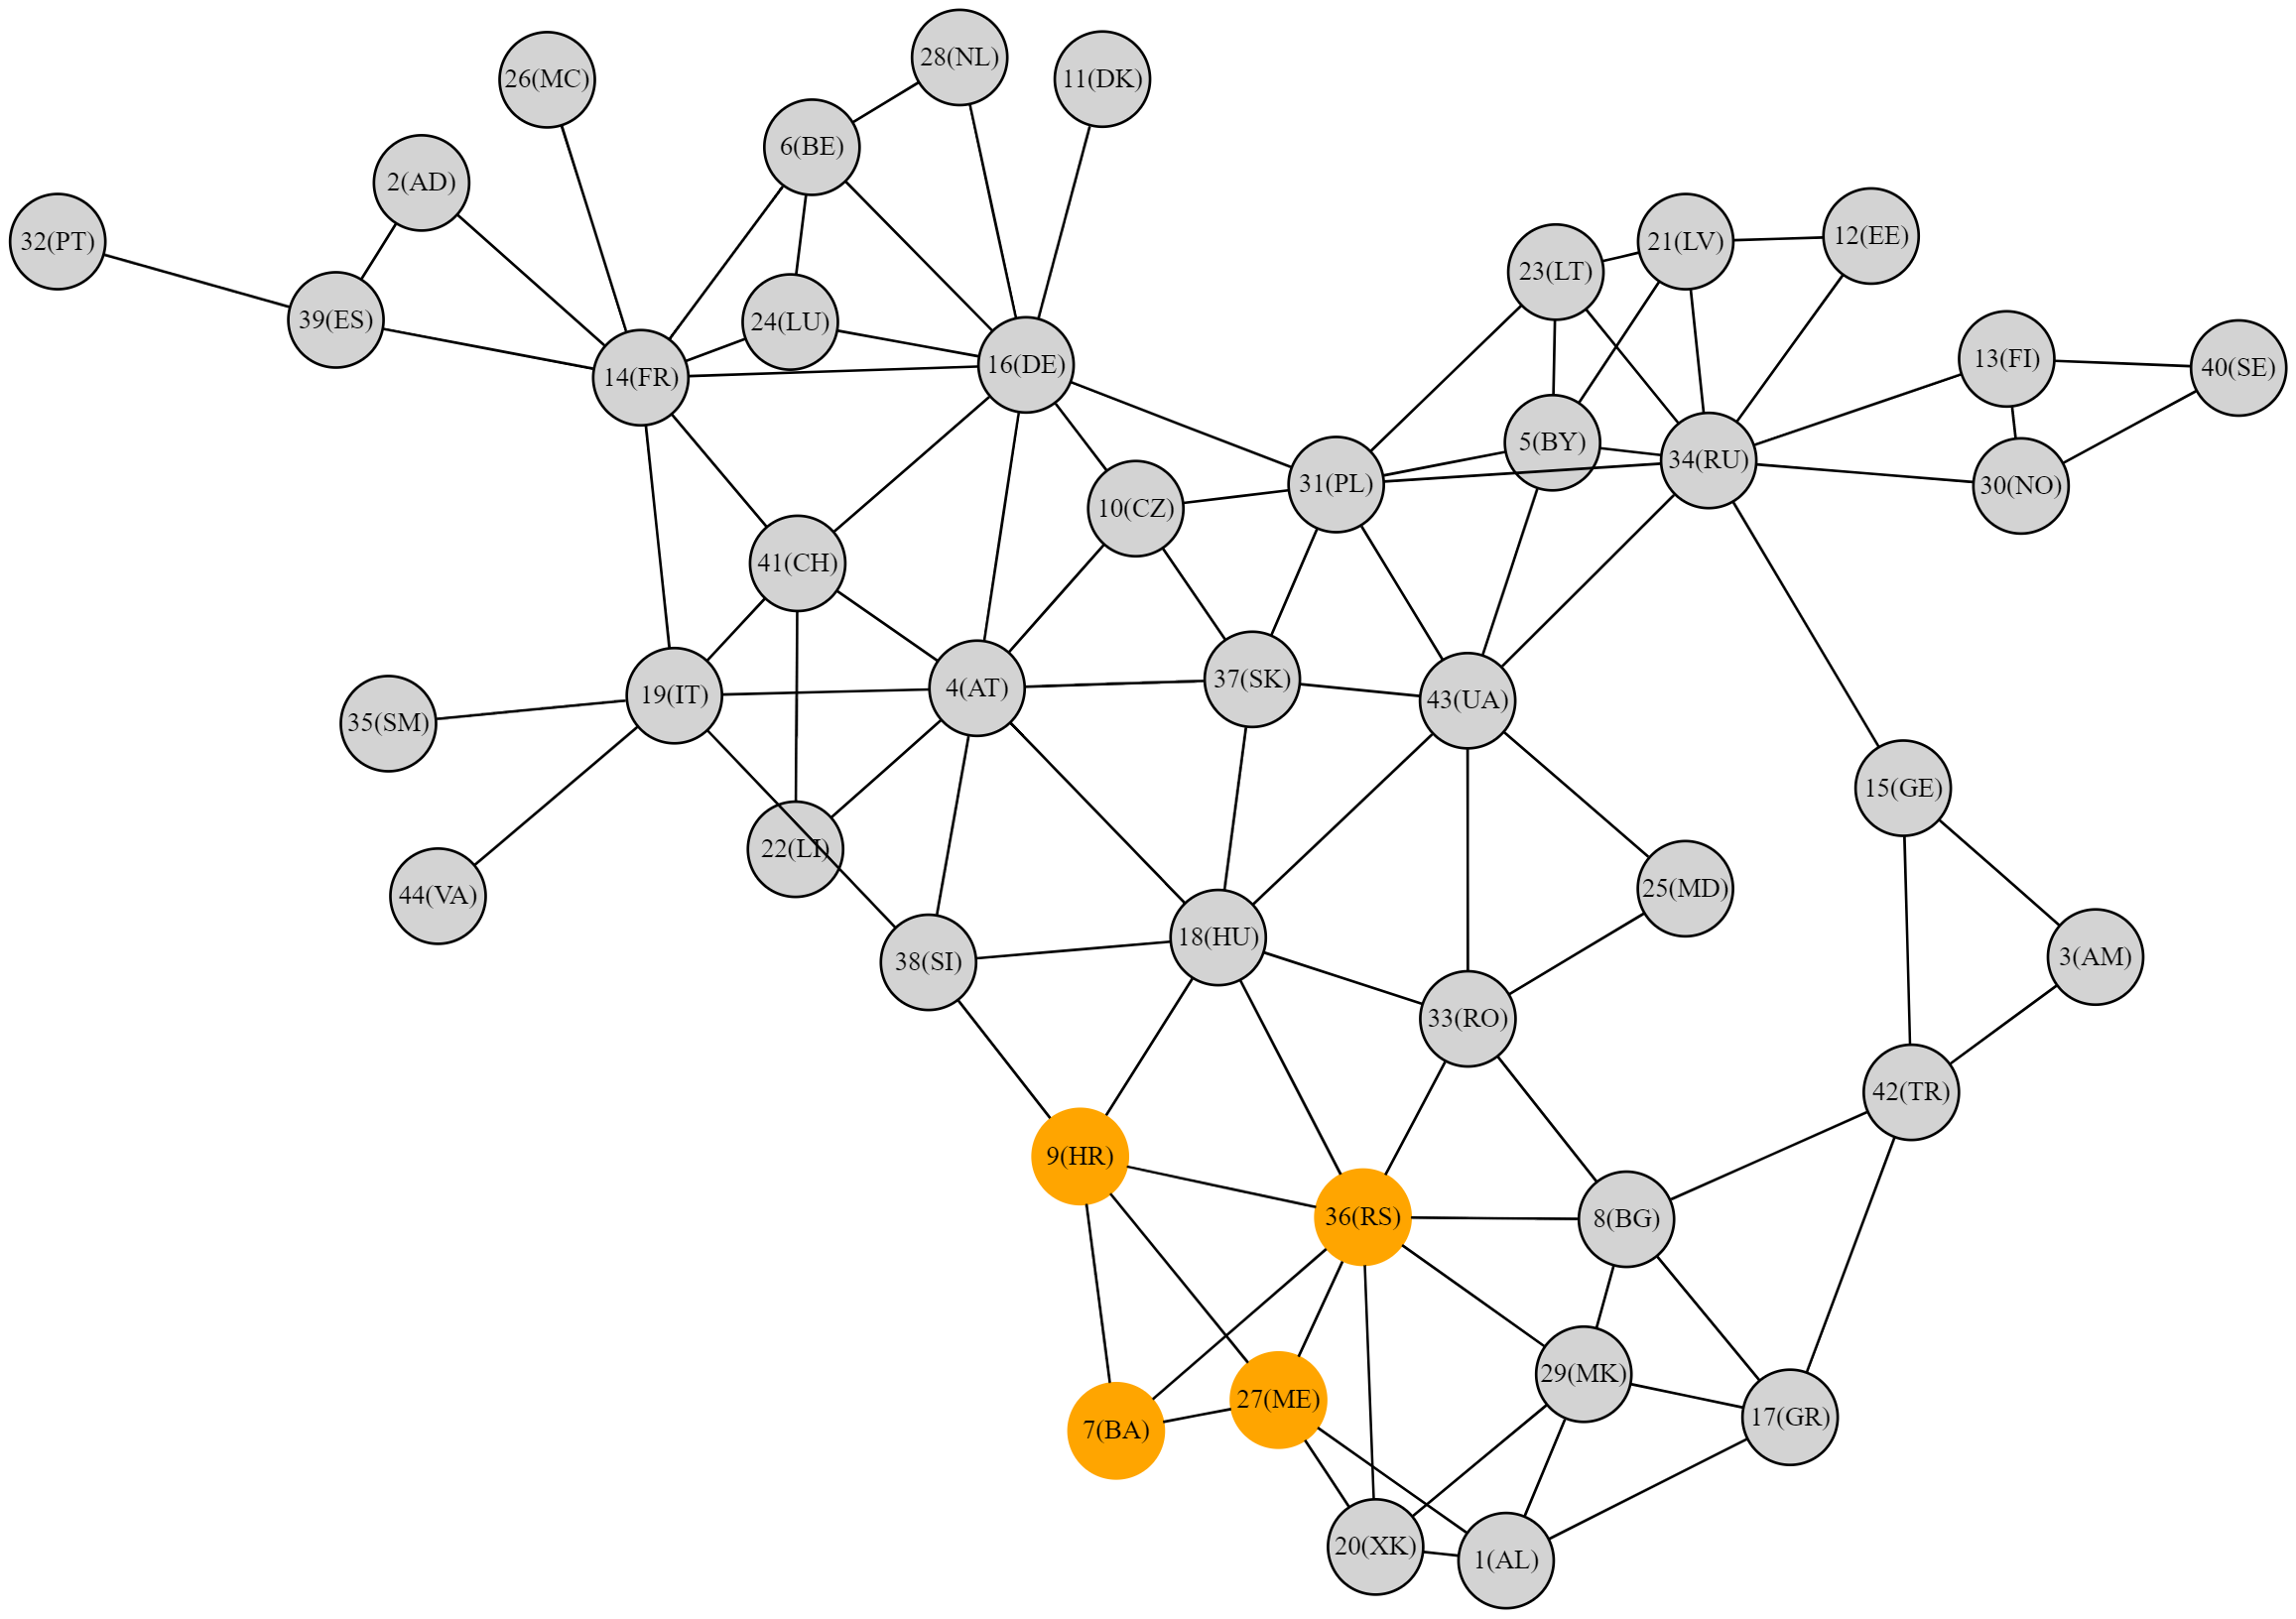
\includegraphics[width=1\textwidth]{clique.png}
		\caption{Maximum clique}
	\end{figure}\newpage
	(f) To find the maximum stable set via MiniZinc we'll check that vertices used in this set aren't adjacent. Size of such set is 19.
	\begin{figure}[h]
		\centering
		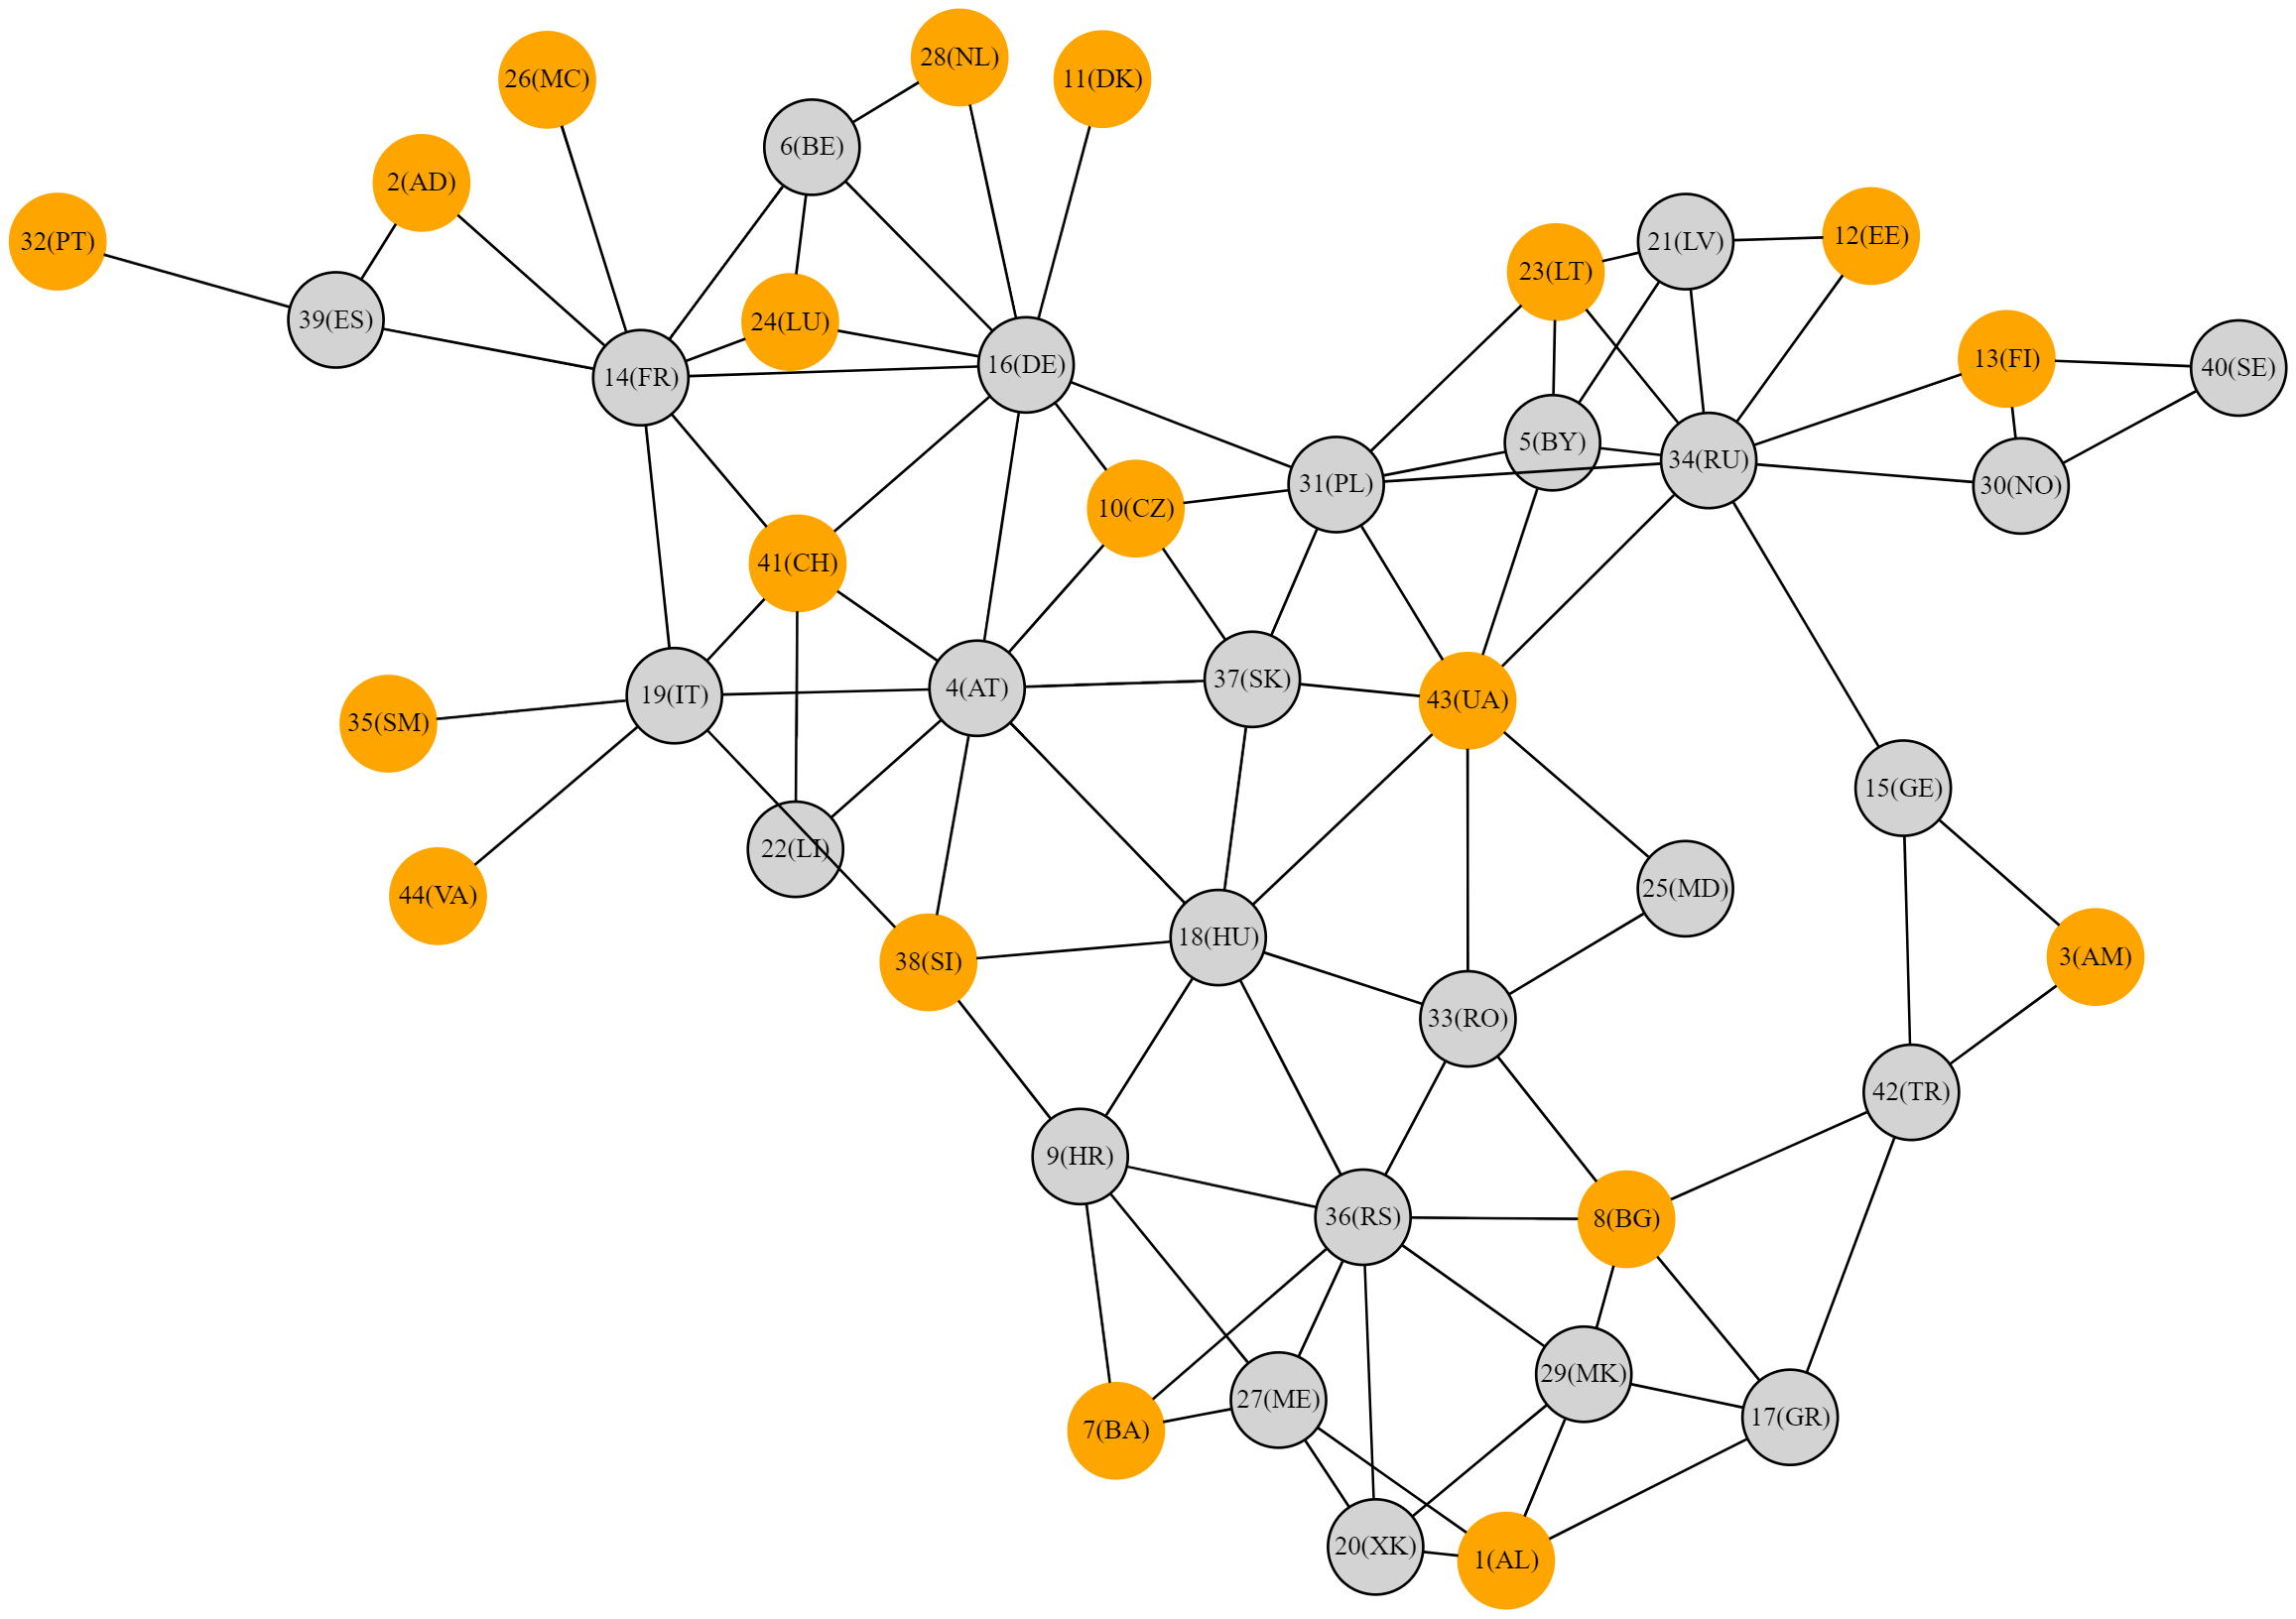
\includegraphics[width=1\textwidth]{stable set.png}
		\caption{Maximum stable set}
	\end{figure}\newpage
	(g) To find the maximum matching via MiniZinc we'll check that edges used in this set aren't adjacent. Size of such matching is 20.
	\begin{figure}[h]
		\centering
		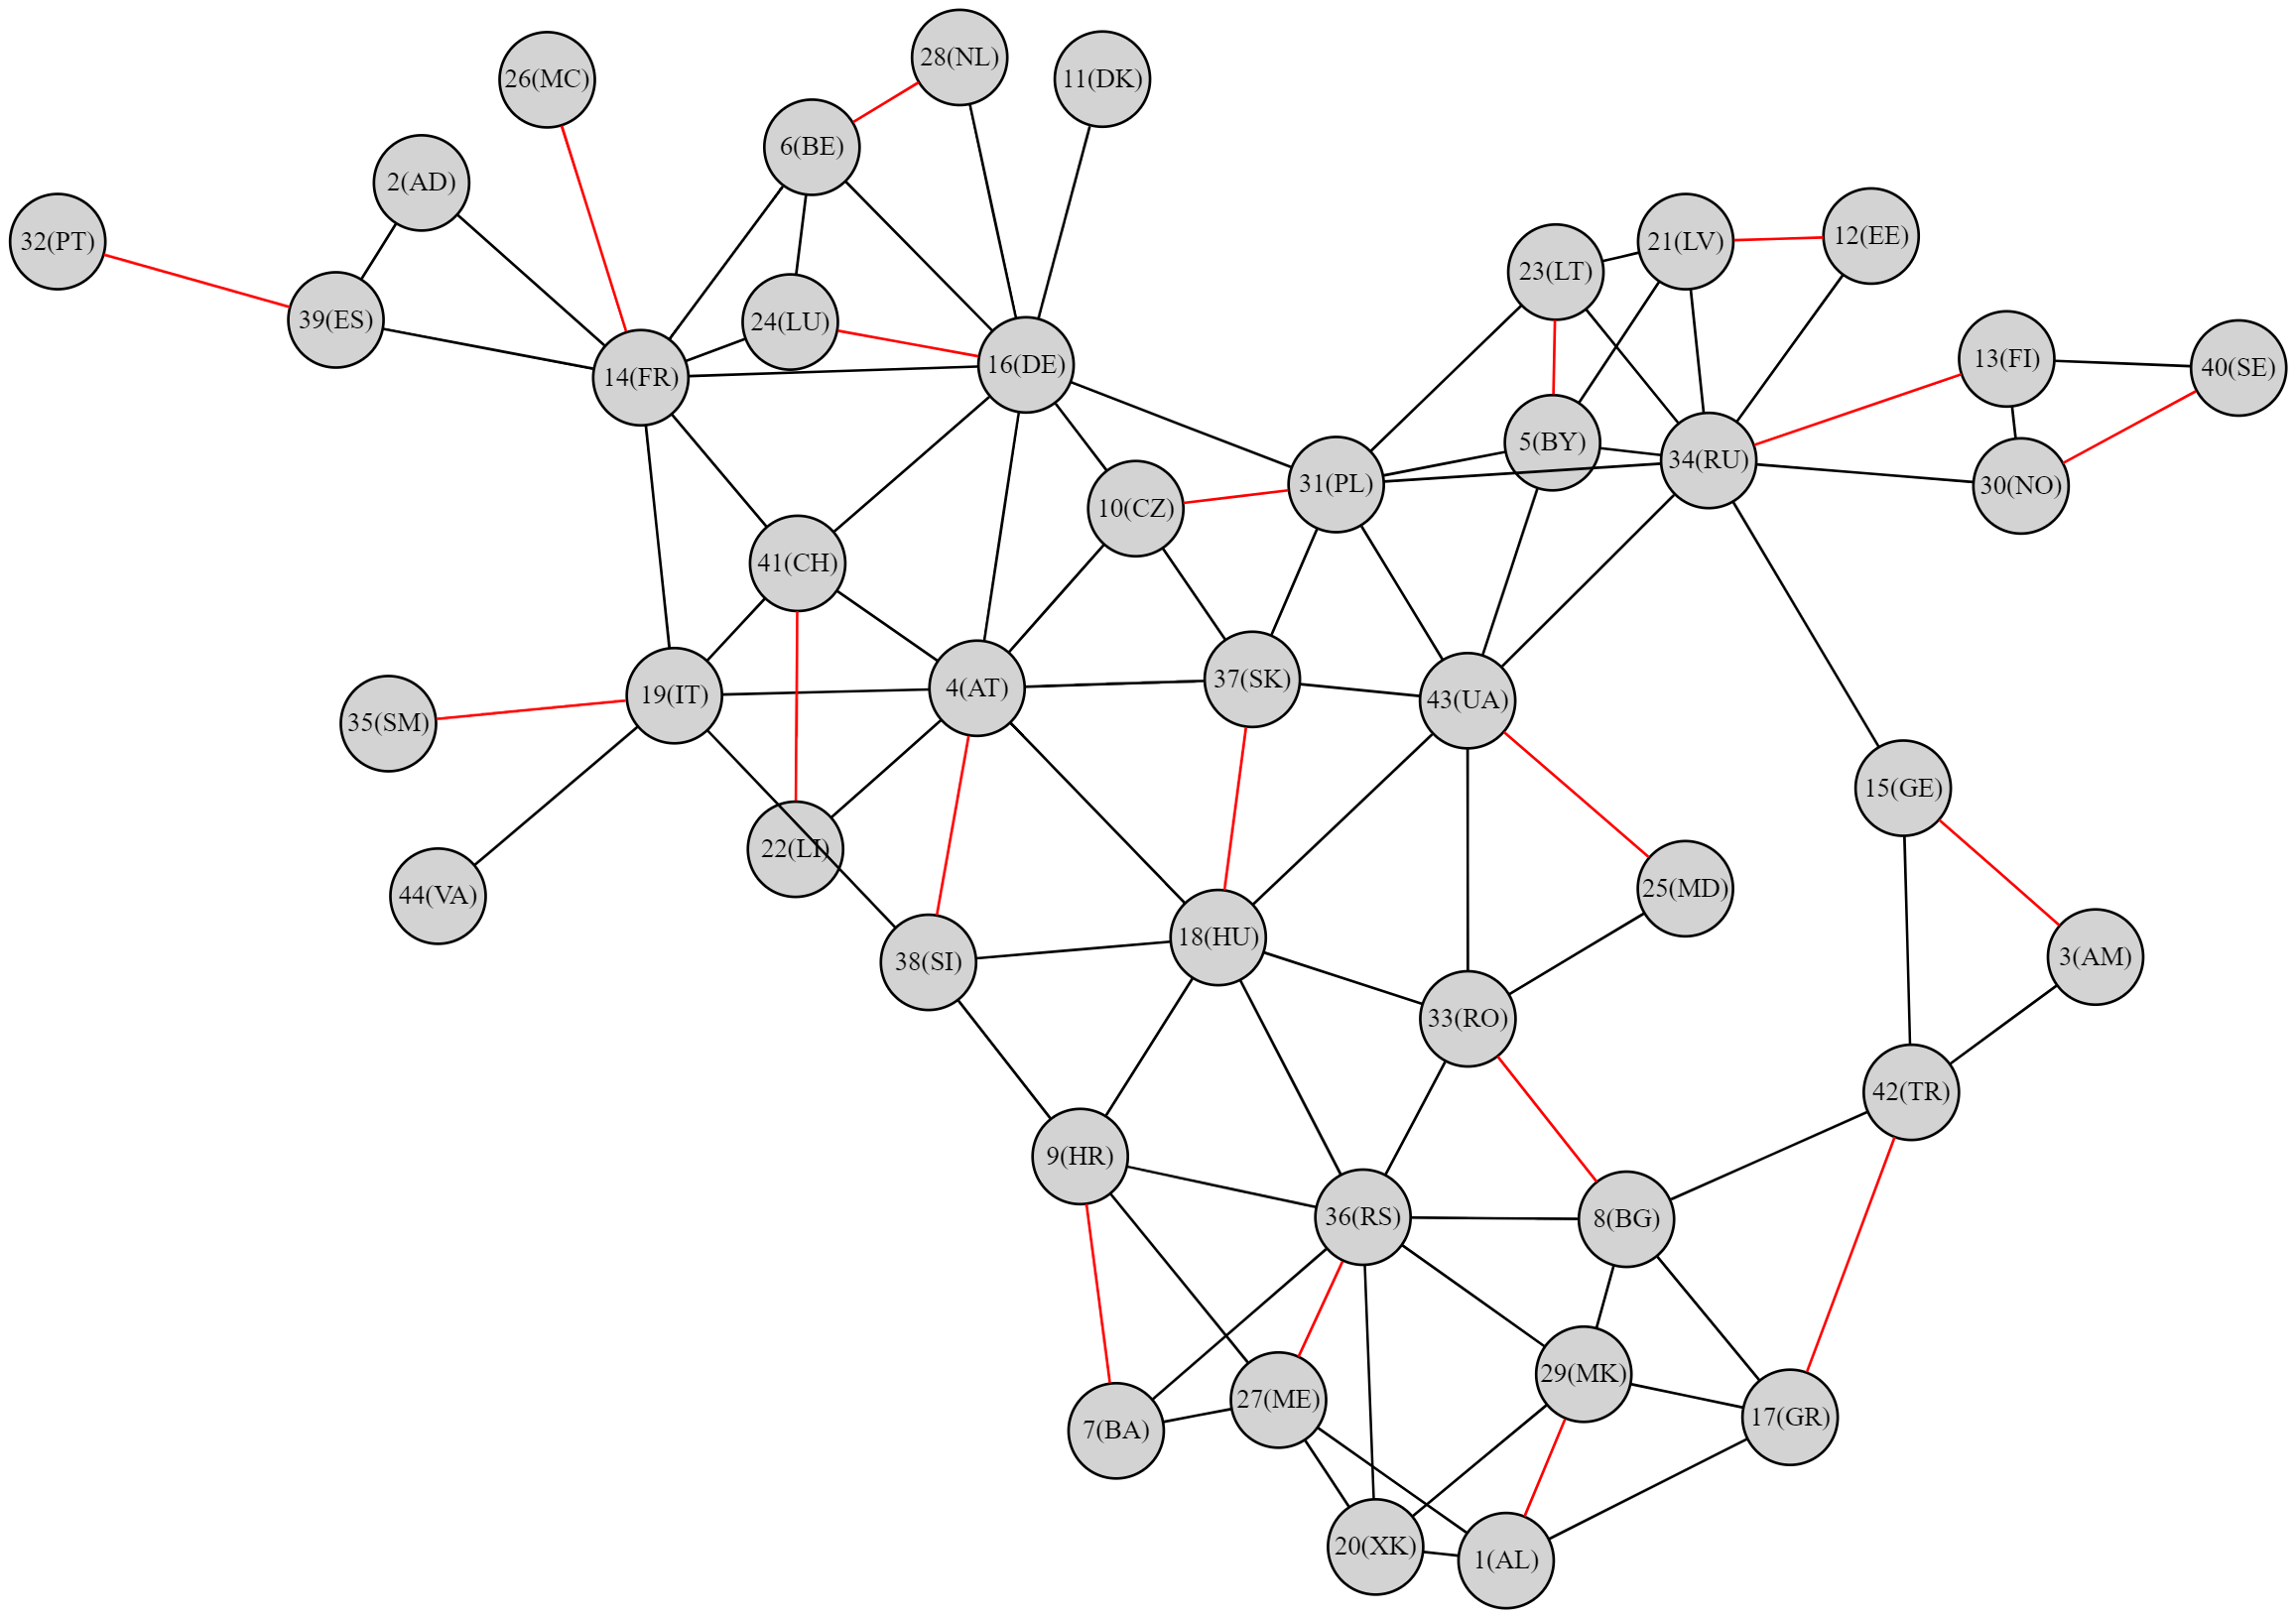
\includegraphics[width=1\textwidth]{matching.png}
		\caption{Maximum matching}
	\end{figure}\newpage
	(h) To find the minimum vertex cover via MiniZinc we'll check that for every edje in the graph at least one of its incident vertives is in this set. Size of such set is 25.
	\begin{figure}[h]
		\centering
		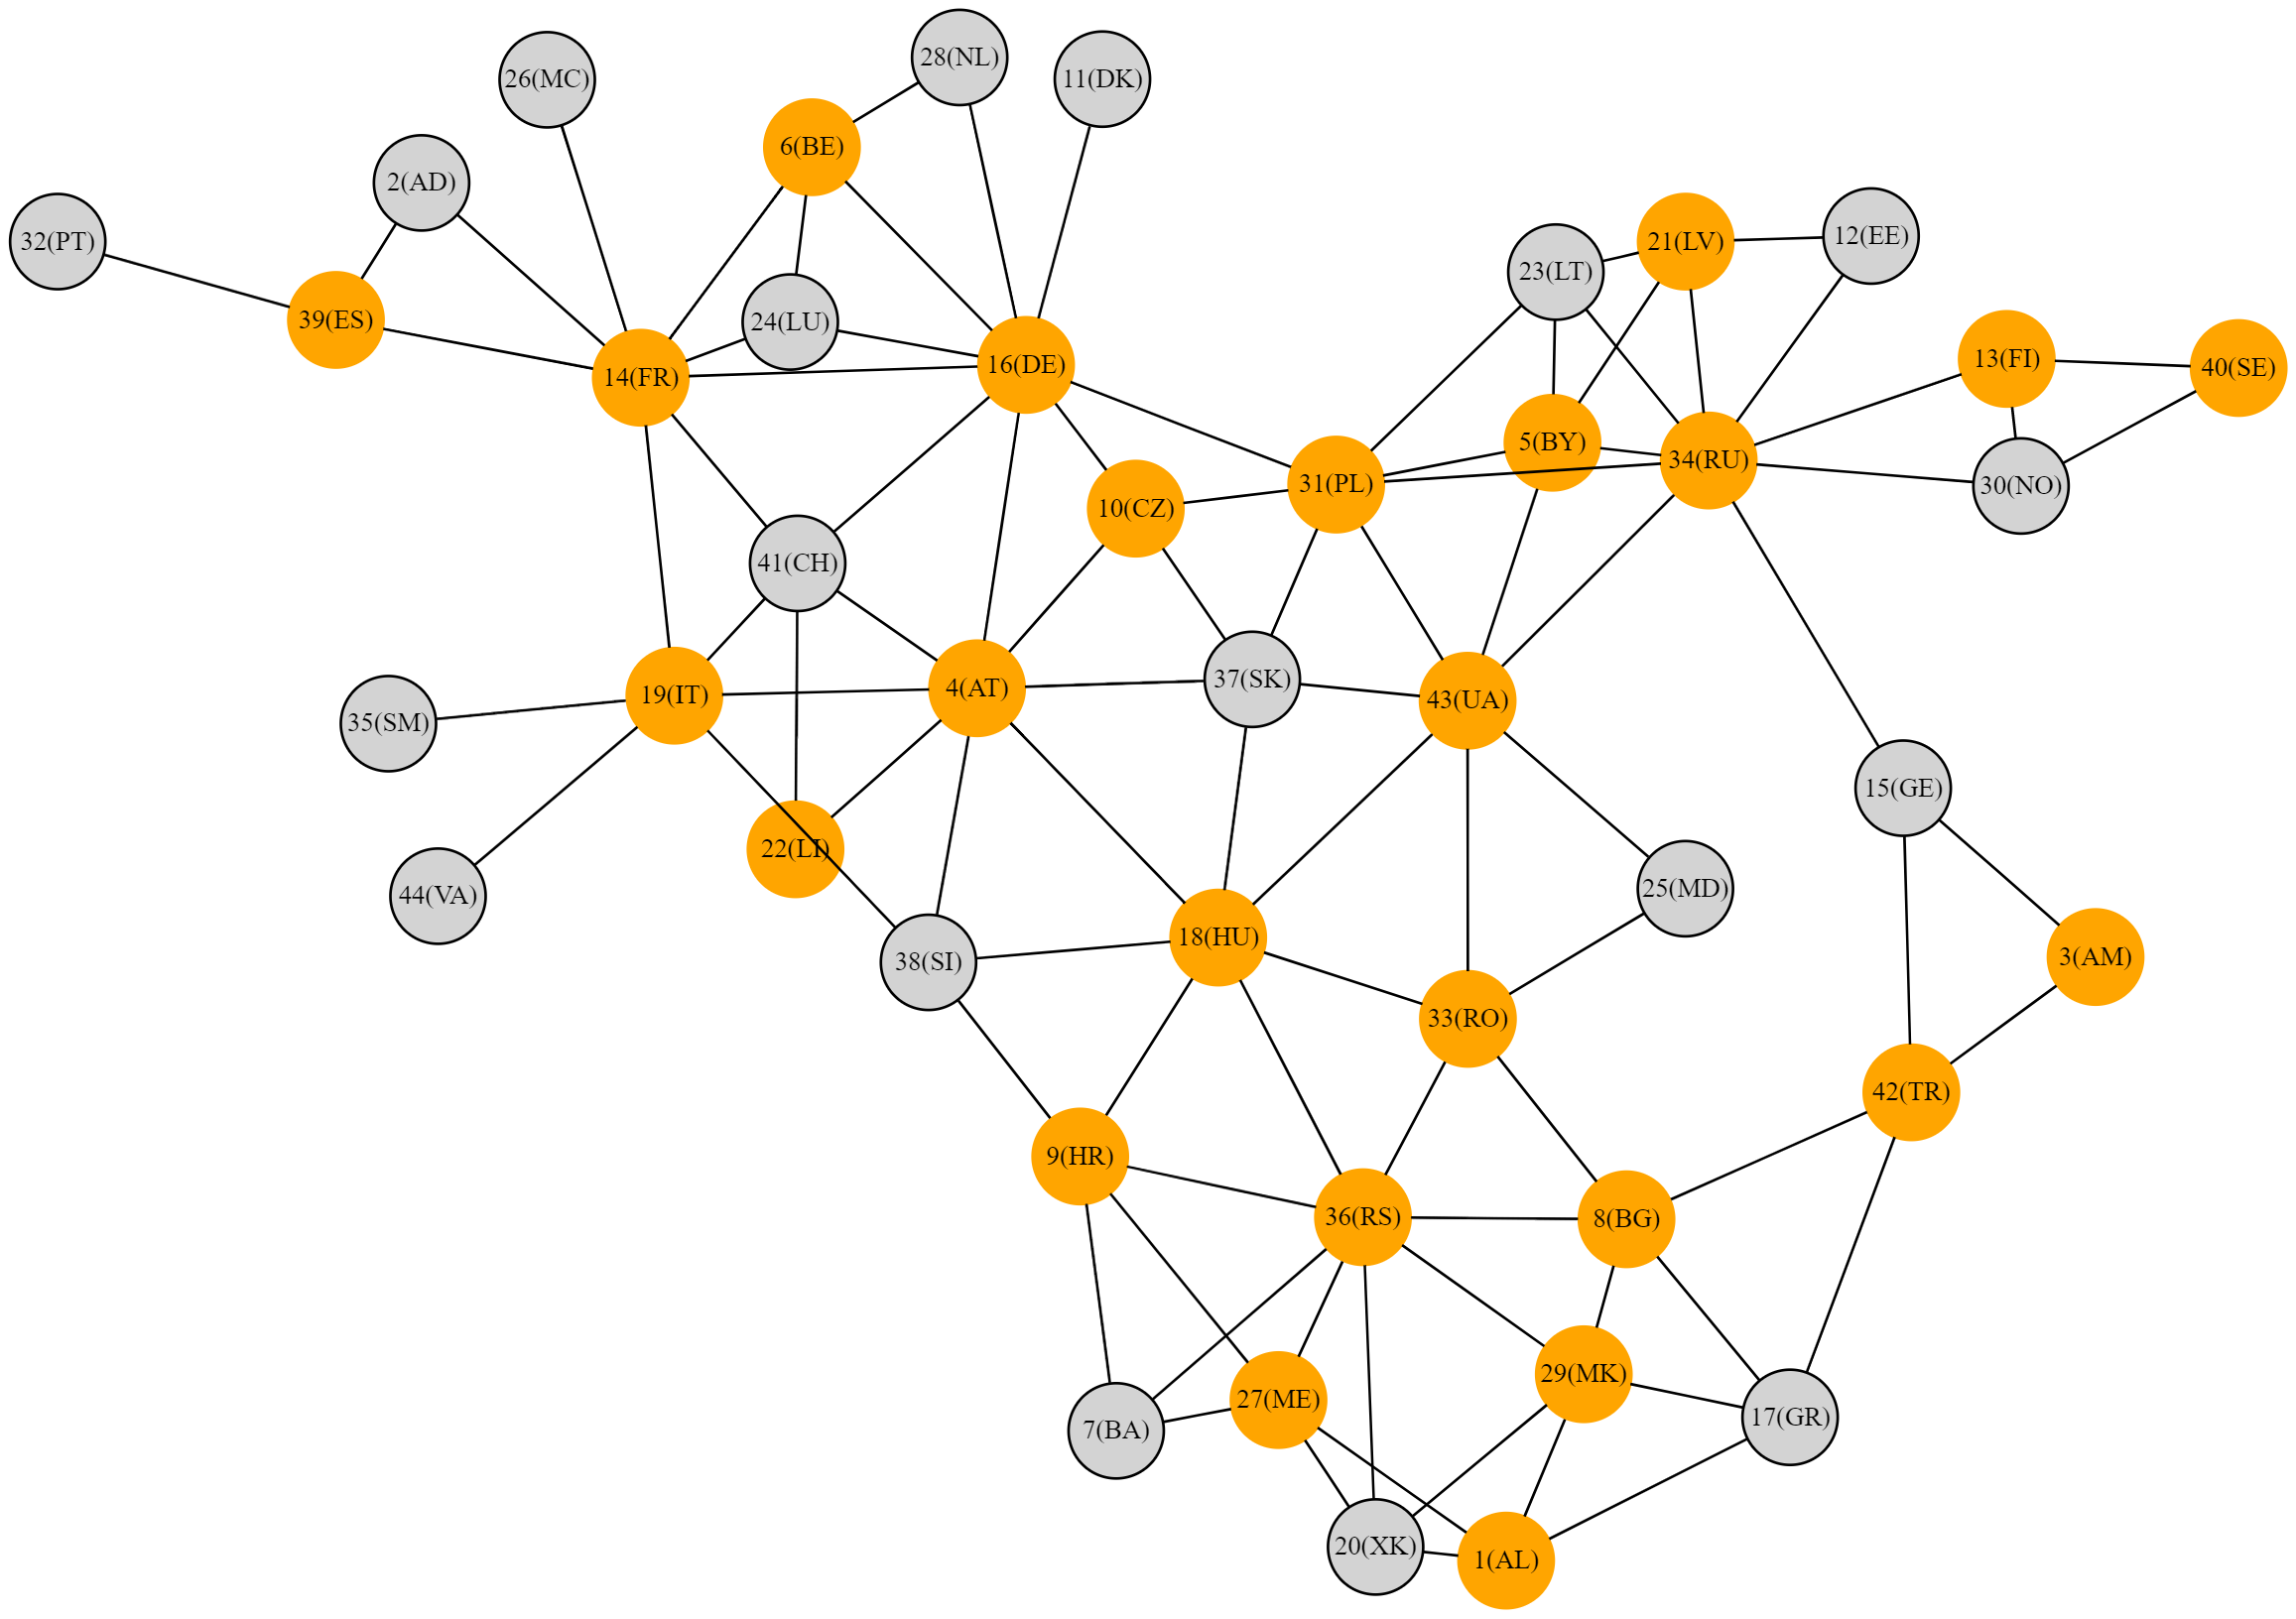
\includegraphics[width=1\textwidth]{v_cover.png}
		\caption{Minimum vertex cover}
	\end{figure}\newpage
	(i) To find the minimum edge cover via MiniZinc we'll check that every vertex in the graph is incident to at least 1 edge from this set. Size of such set is 24.
	\begin{figure}[h]
		\centering
		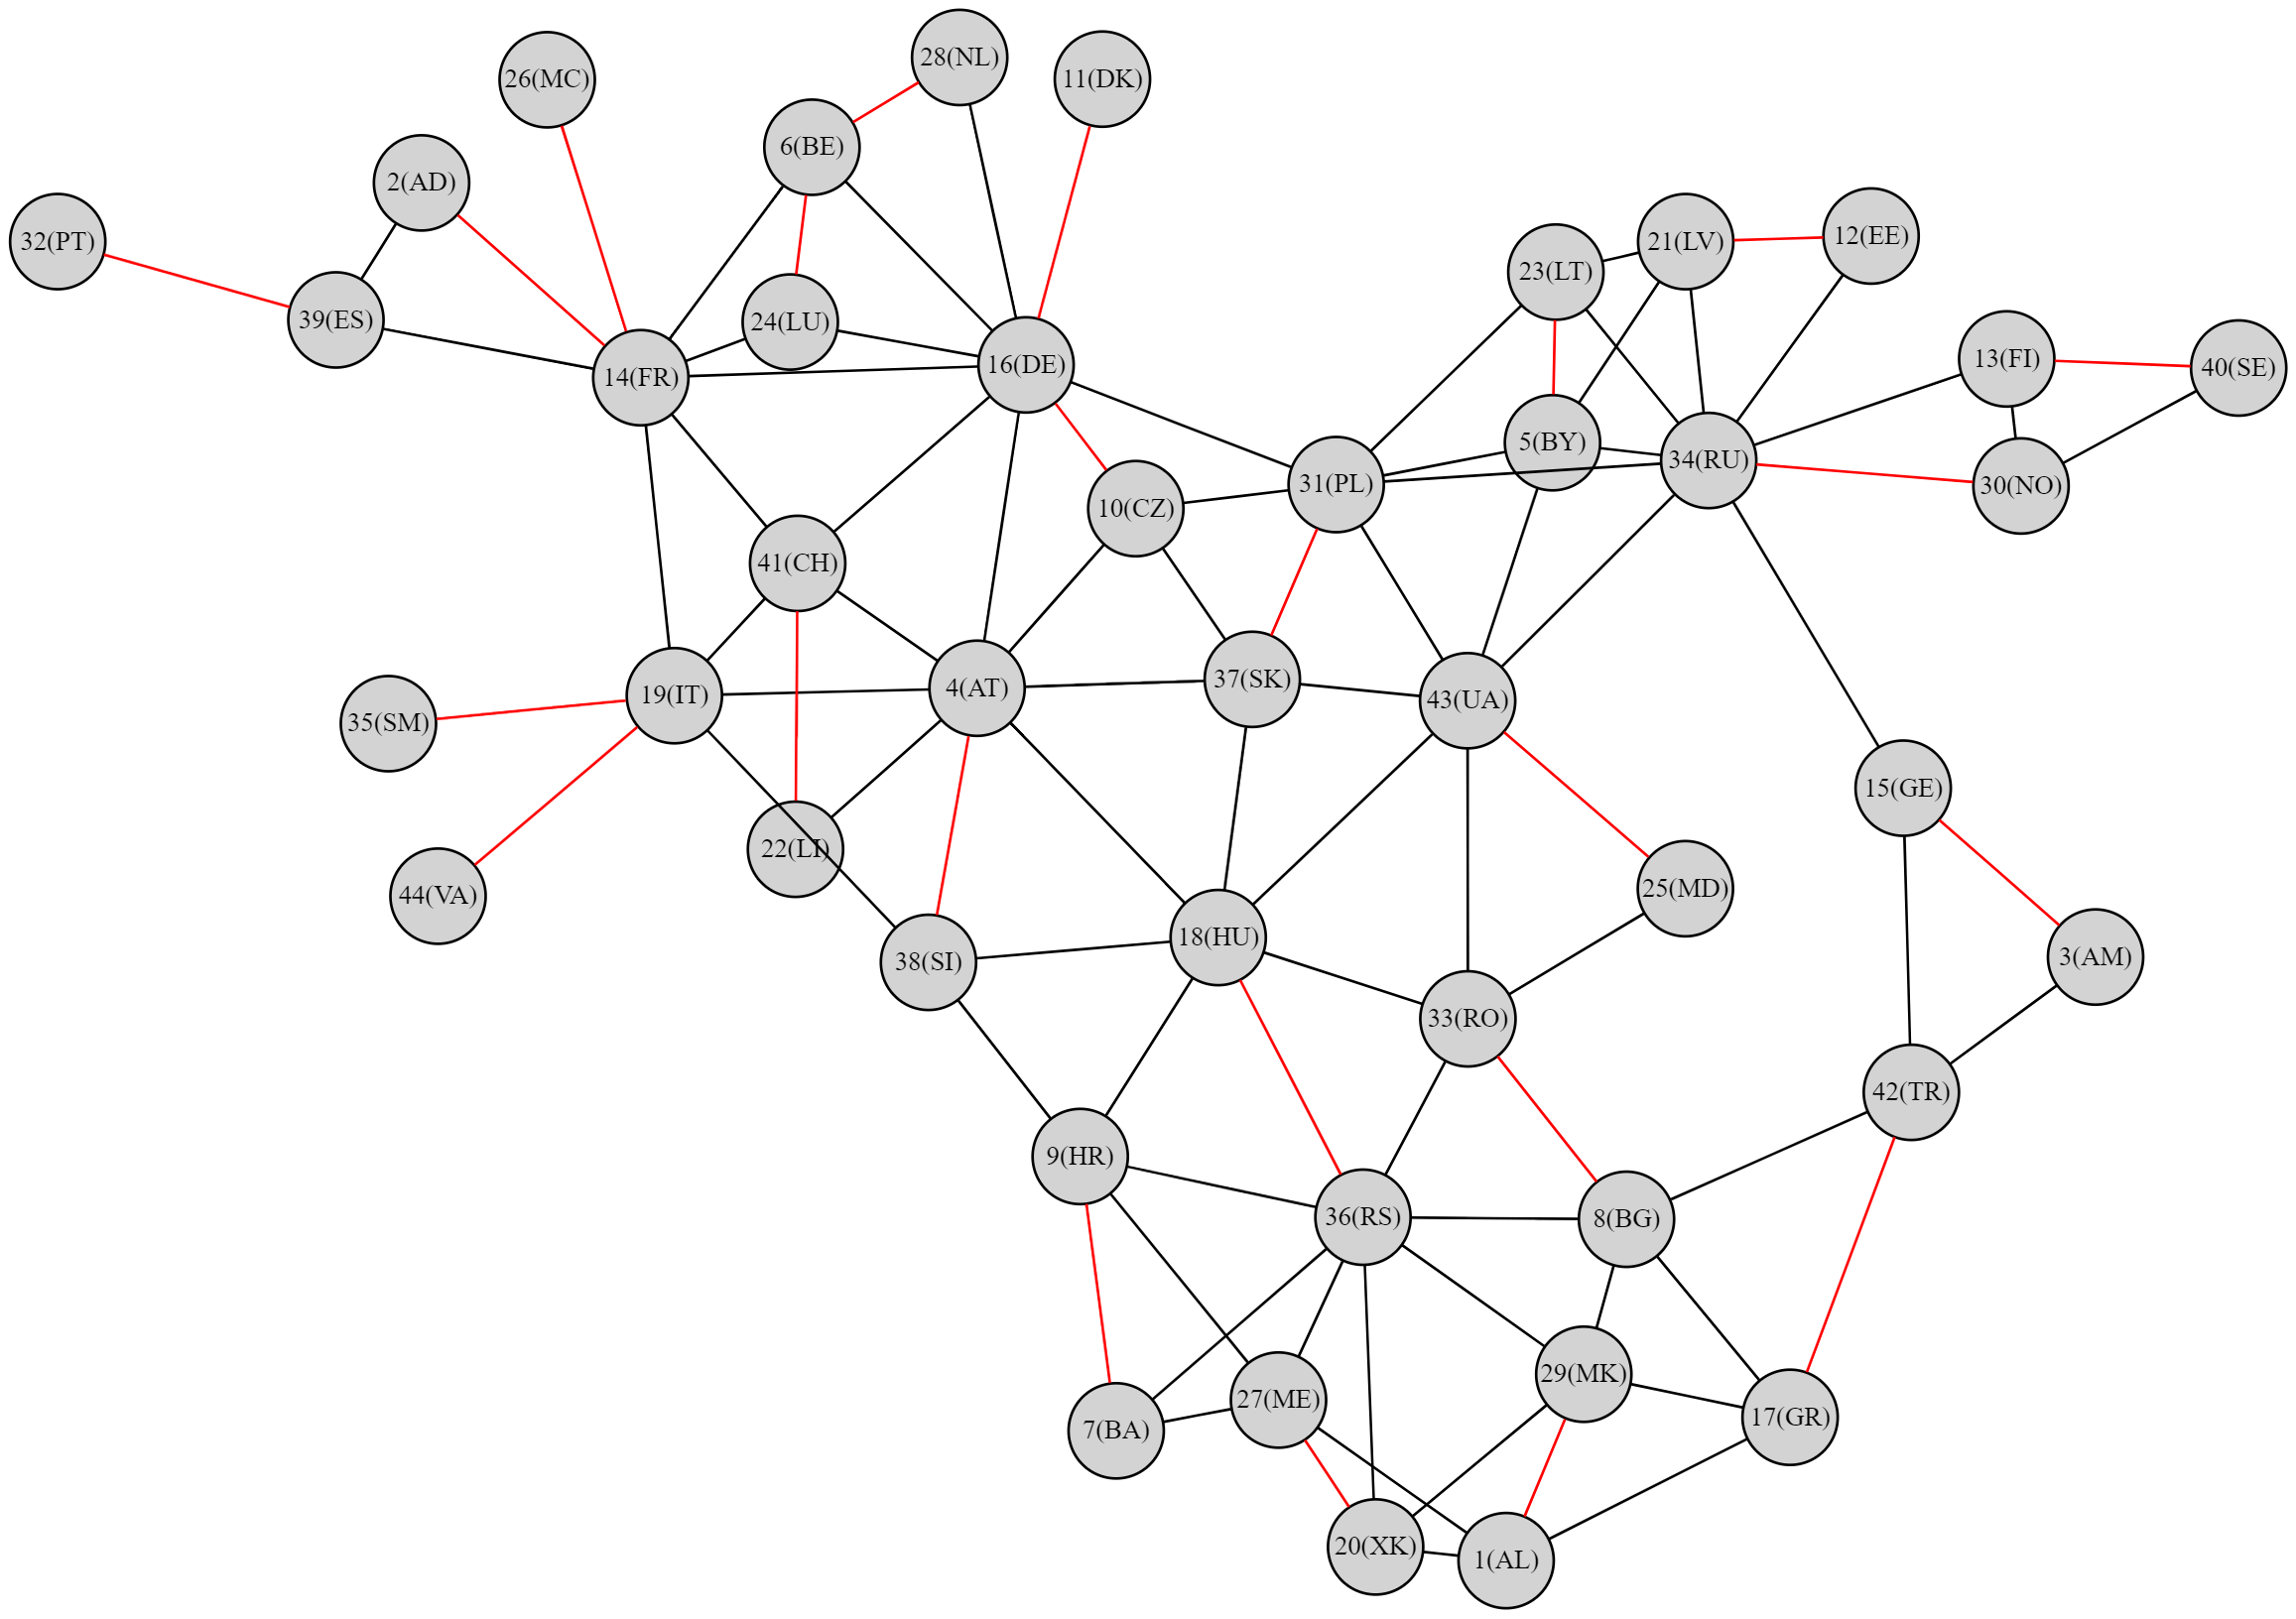
\includegraphics[width=1\textwidth]{ecover.png}
		\caption{Minimum edge cover}
	\end{figure}\newpage
	(j) At first we'll consider subgraph of $\mathcal{G}$, induced on all vertices except those which are highlighted in blue. In such subgraph we can find Hamiltonian cycle of size 34 -- its edges are highlighted in red. It's impossible to add blue vertices to this cycle in $\mathcal{G}$ to make it Hamiltonian in $\mathcal{G}$ because they're connected to subgraph only by cut vertices. We can still add purple edges to the cycle to make from it the walk that visits all vertices. We have to use IT-SM, IT-VA, FR-MC, DE-DK, ES-PT twice as they're bridges. To add other blue vertices we need $3 + 4 = 7$ more edges (it's easy to find shortest walks in these little subgraphs -- we have few edges to search through). So the length of the shortest walk that visits all vertices is 51.
	\begin{figure}[h]
		\centering
		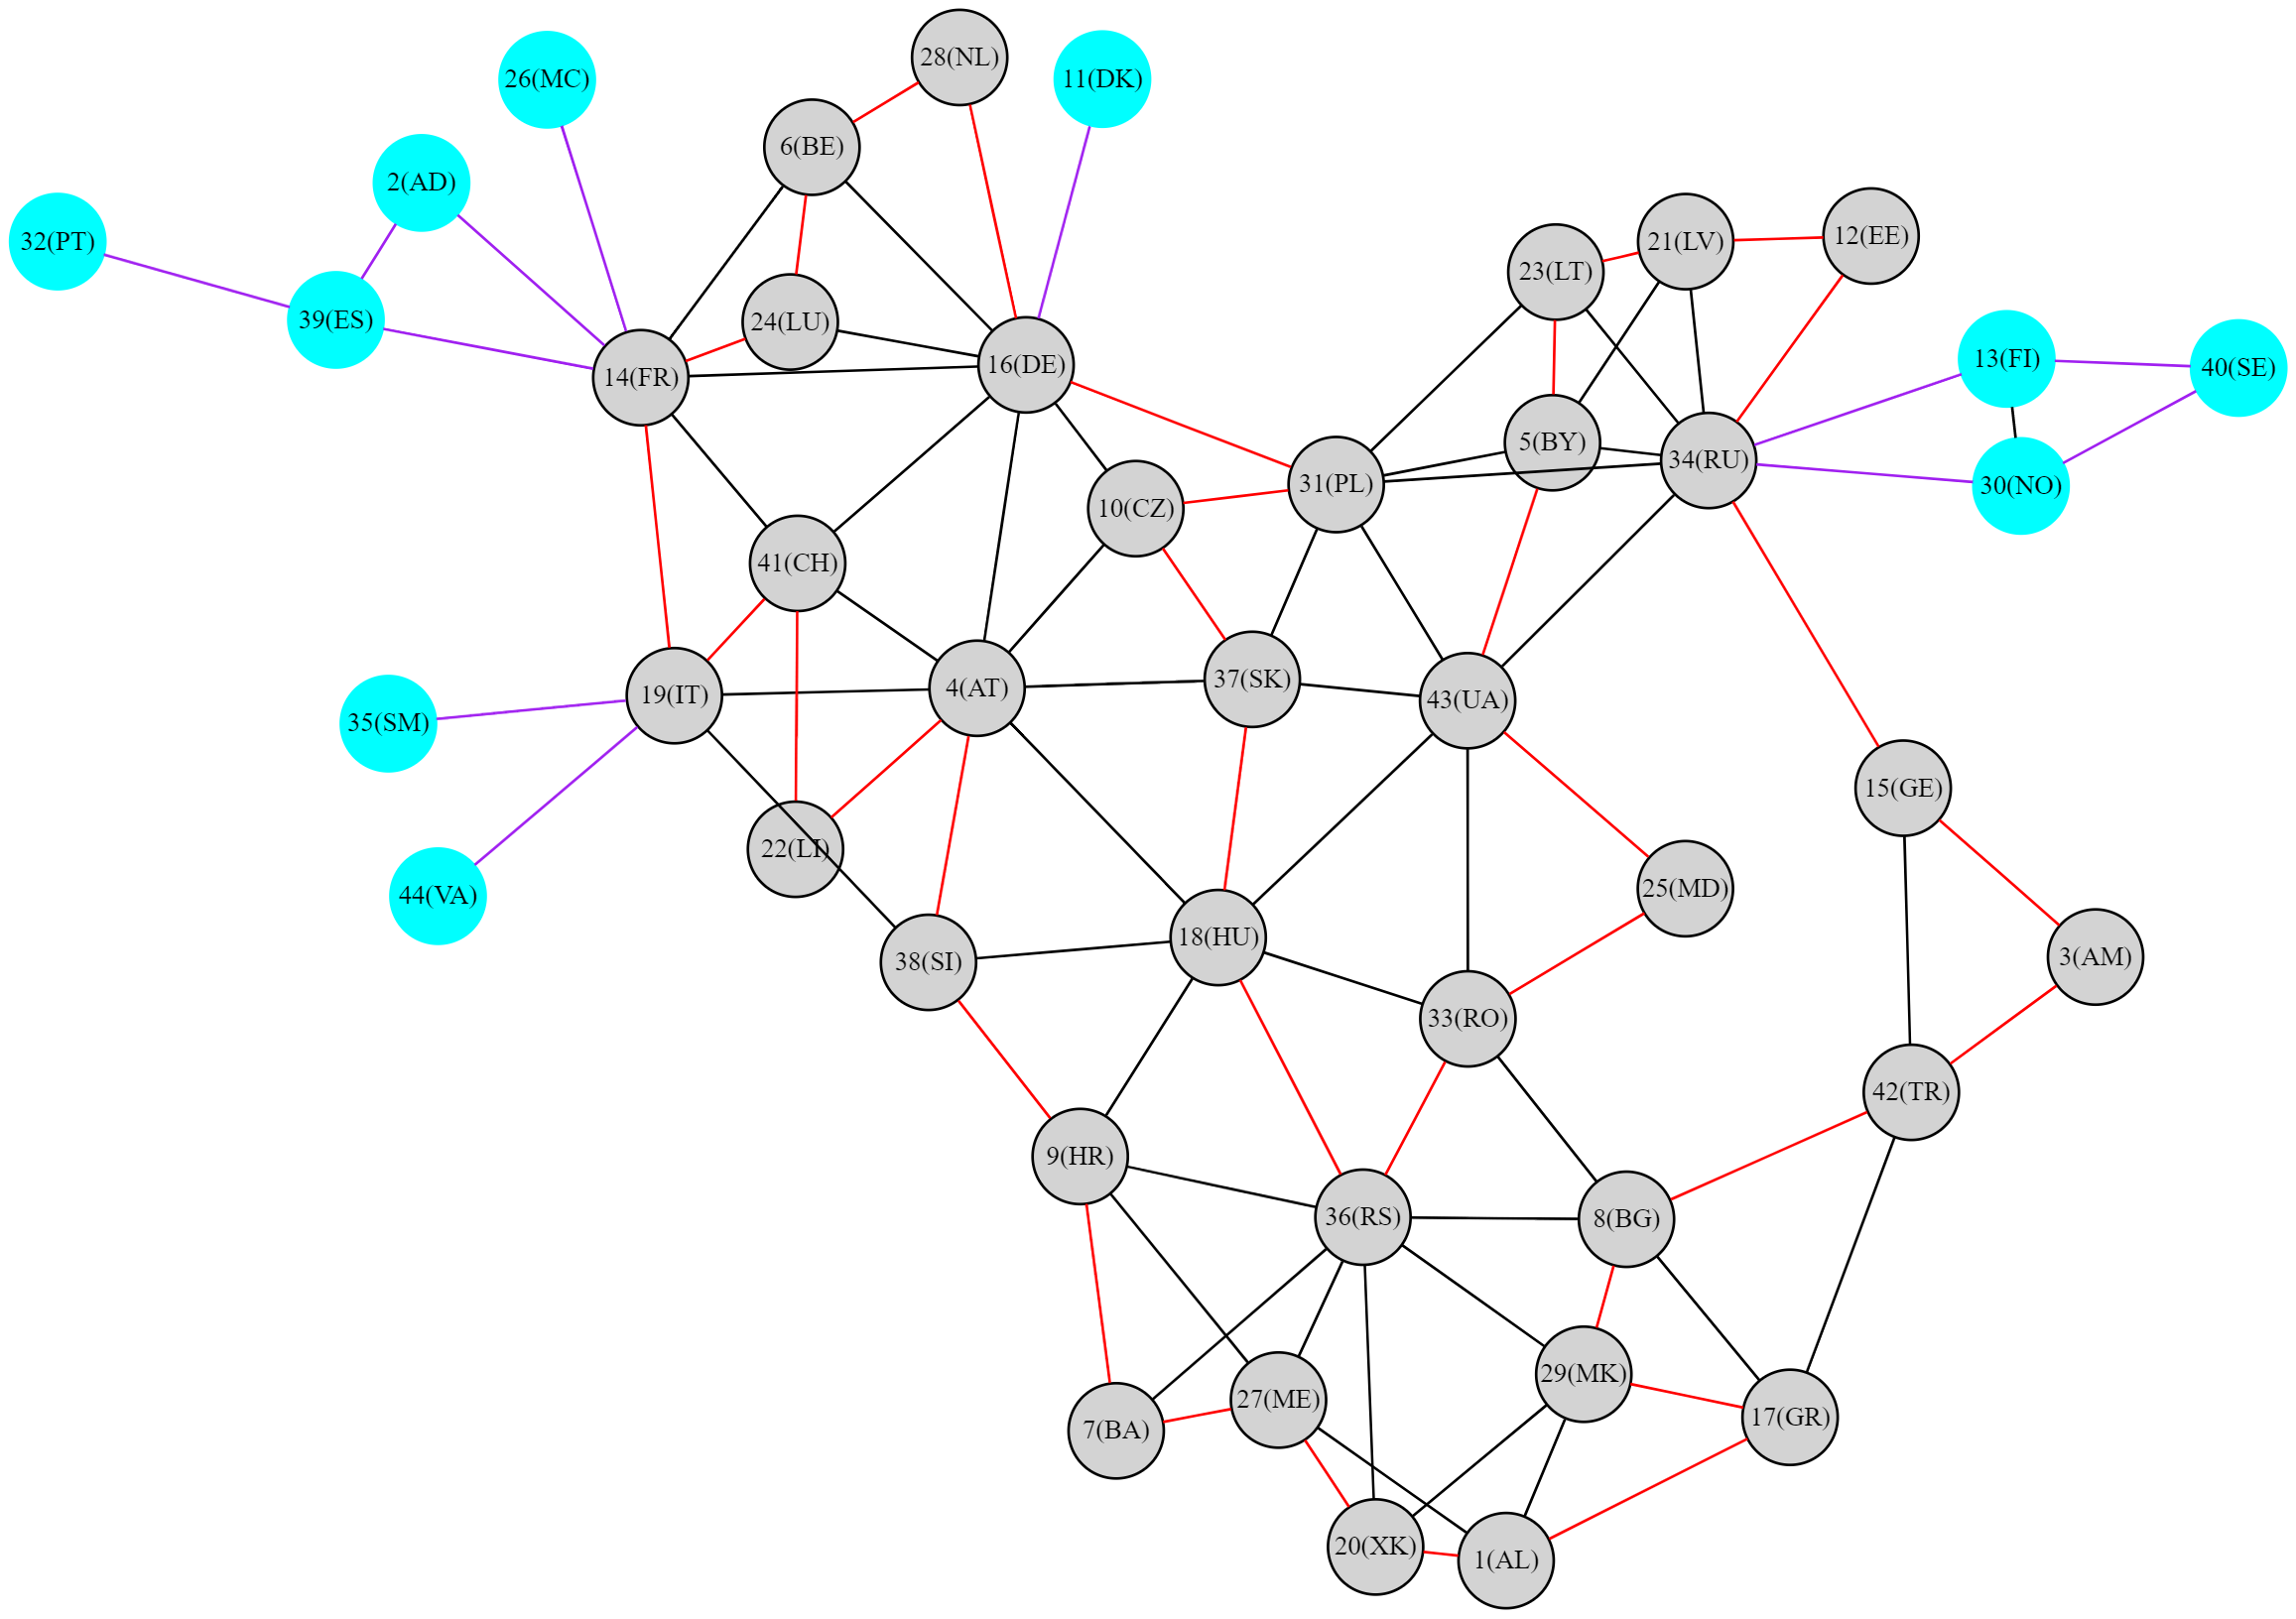
\includegraphics[width=1\textwidth]{v_walk.png}
		\caption{Shortest 'vertex' walk}
	\end{figure}\newpage
	(k)  If all vertices had even degrees, it would be possible to visit all edges using an Eulerian cycle, but since there are many vertices of odd degree, for every vertex of odd degree there is at least one incident edge which will be used twice. So we'll try to minimize number of such edges. In the end we manually get the walk. It has length of 110 and its vertices sequence is:\par
	\texttt{34 13 40 30 13 30 34 12 21 23 34 21 5 23 31 5 34 31 16 11 16 28 6 14 26 14 2 39 32 39
	14 24 6 16 24 16 14 19 35 19 44 19 41 14 41 22 4 41 16 4 19 38 4 10 16 31 10 37 4 18 36 9 18 37 31 43 37 43 5 43 34 43 25 33 43 18 33 8 36 33 18 36 9 27 9 7 27 7 36 27 20 1 27 1 29 20 36 29 1 17 29 8 17 42 8 42 3 15 42 15 34}
	\begin{figure}[h]
		\centering
		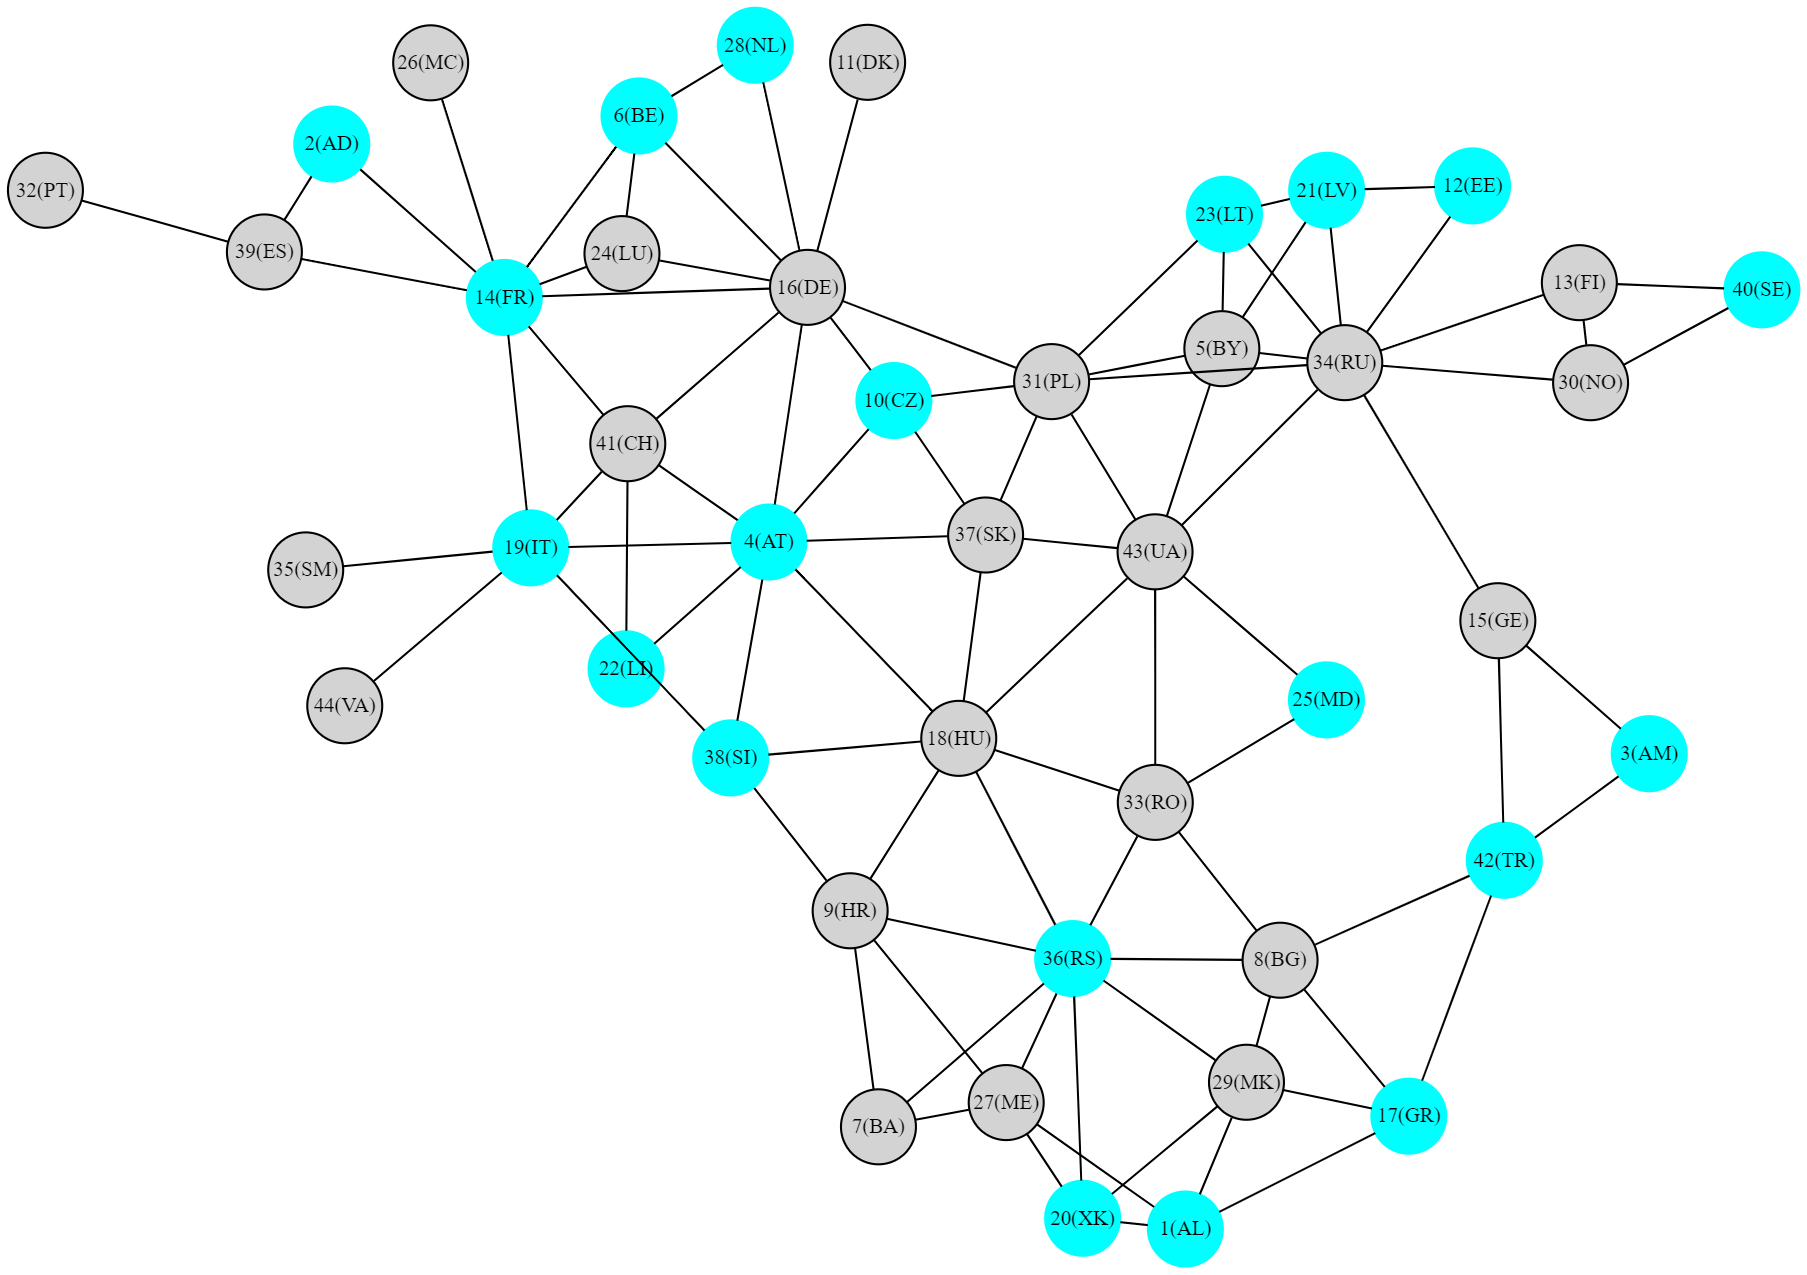
\includegraphics[width=1\textwidth]{even.png}
		\caption{Even degree vertices are cyan}
	\end{figure}\newpage
	\newpage
	(l) Here we'll consider biconnectivity relation as relation on $E^2$, where the edges of a block belong to one equivalence class if subgraph on them and their incident vertices is maximal 2-vertex-connected or it's $K_2$ and doesn't belong to 2-vertex-connected subgraph. Then all we need to do is manually find cut vertices for each connected component and split connected components into blocks (blocks share no or only cut vertices). There are a total of 9 blocks here. \\\\
	As one block is disconnected from the graph it is only possible to draw separated block-cut trees. Block-cut tree of GB-IE block is $K_1$, so it makes sense to draw block-cut tree of $\mathcal{G}$.
	\begin{figure}[h]
		\centering
		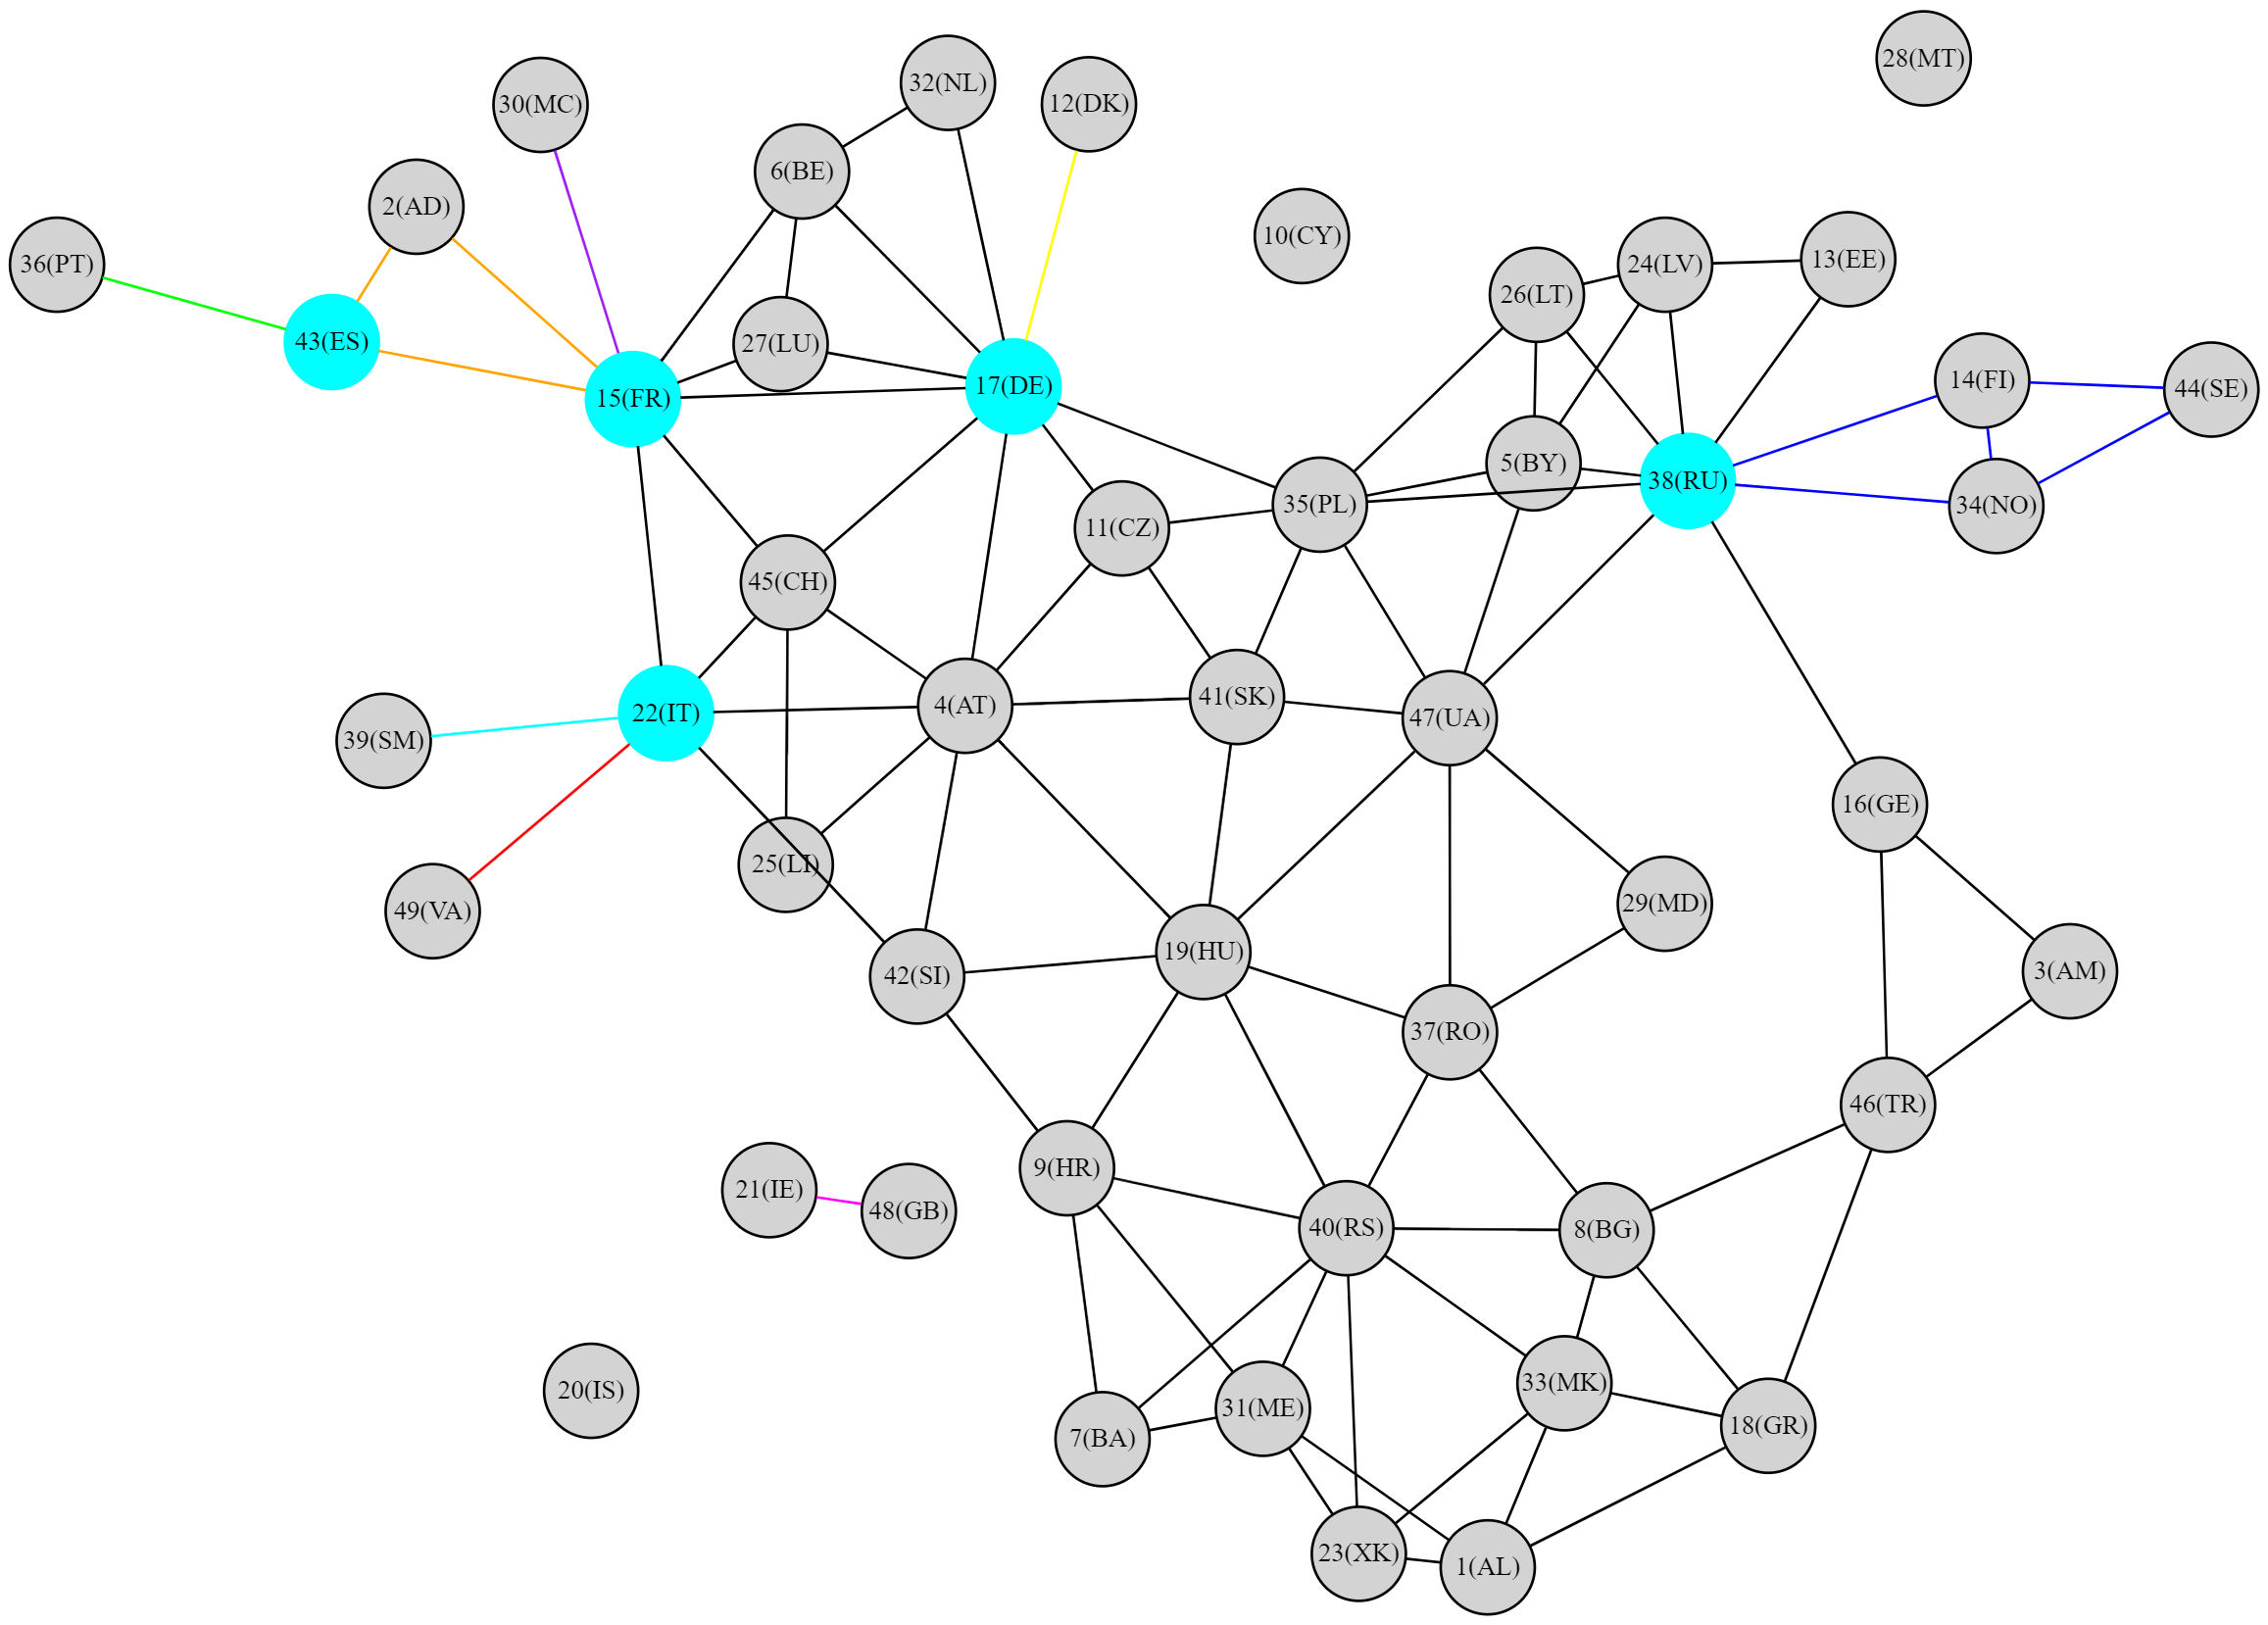
\includegraphics[width=1\textwidth]{blocks.png}
		\caption{Cut vertices are painted cyan, the edges of one block have the same color(black edges are also in the block)}
	\end{figure}\newpage
	\begin{figure}[h]
	\centering
	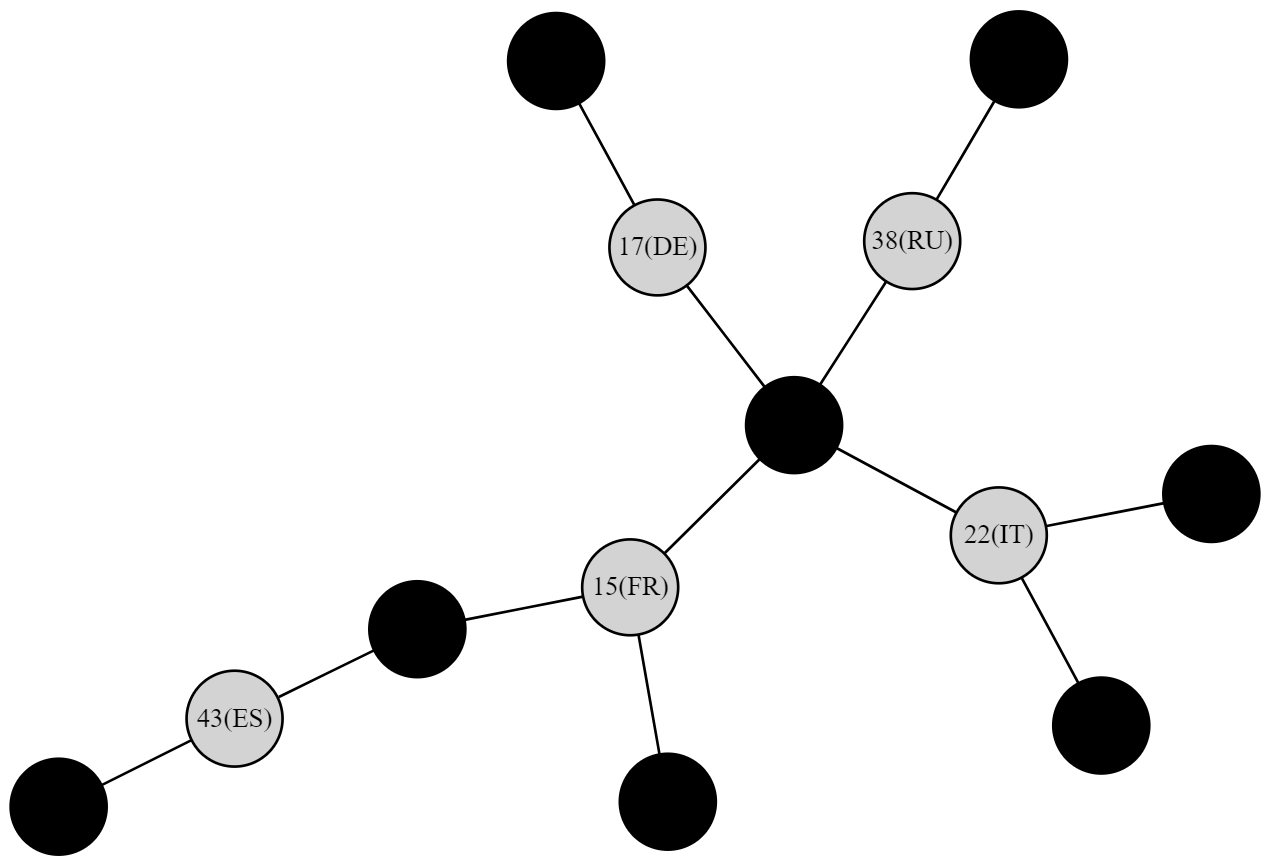
\includegraphics[width=1\textwidth]{block cut tree.png}
	\caption{Block-cut of $\mathcal{G}$ (black vertices are blocks, others are cut 	vertices)}
	\end{figure}
	\newpage
	(m) We'll manually find all bridges (it's not so hard to do in this graph) and split graph to 2-edge-connected components.
	\begin{figure}[h]
		\centering
		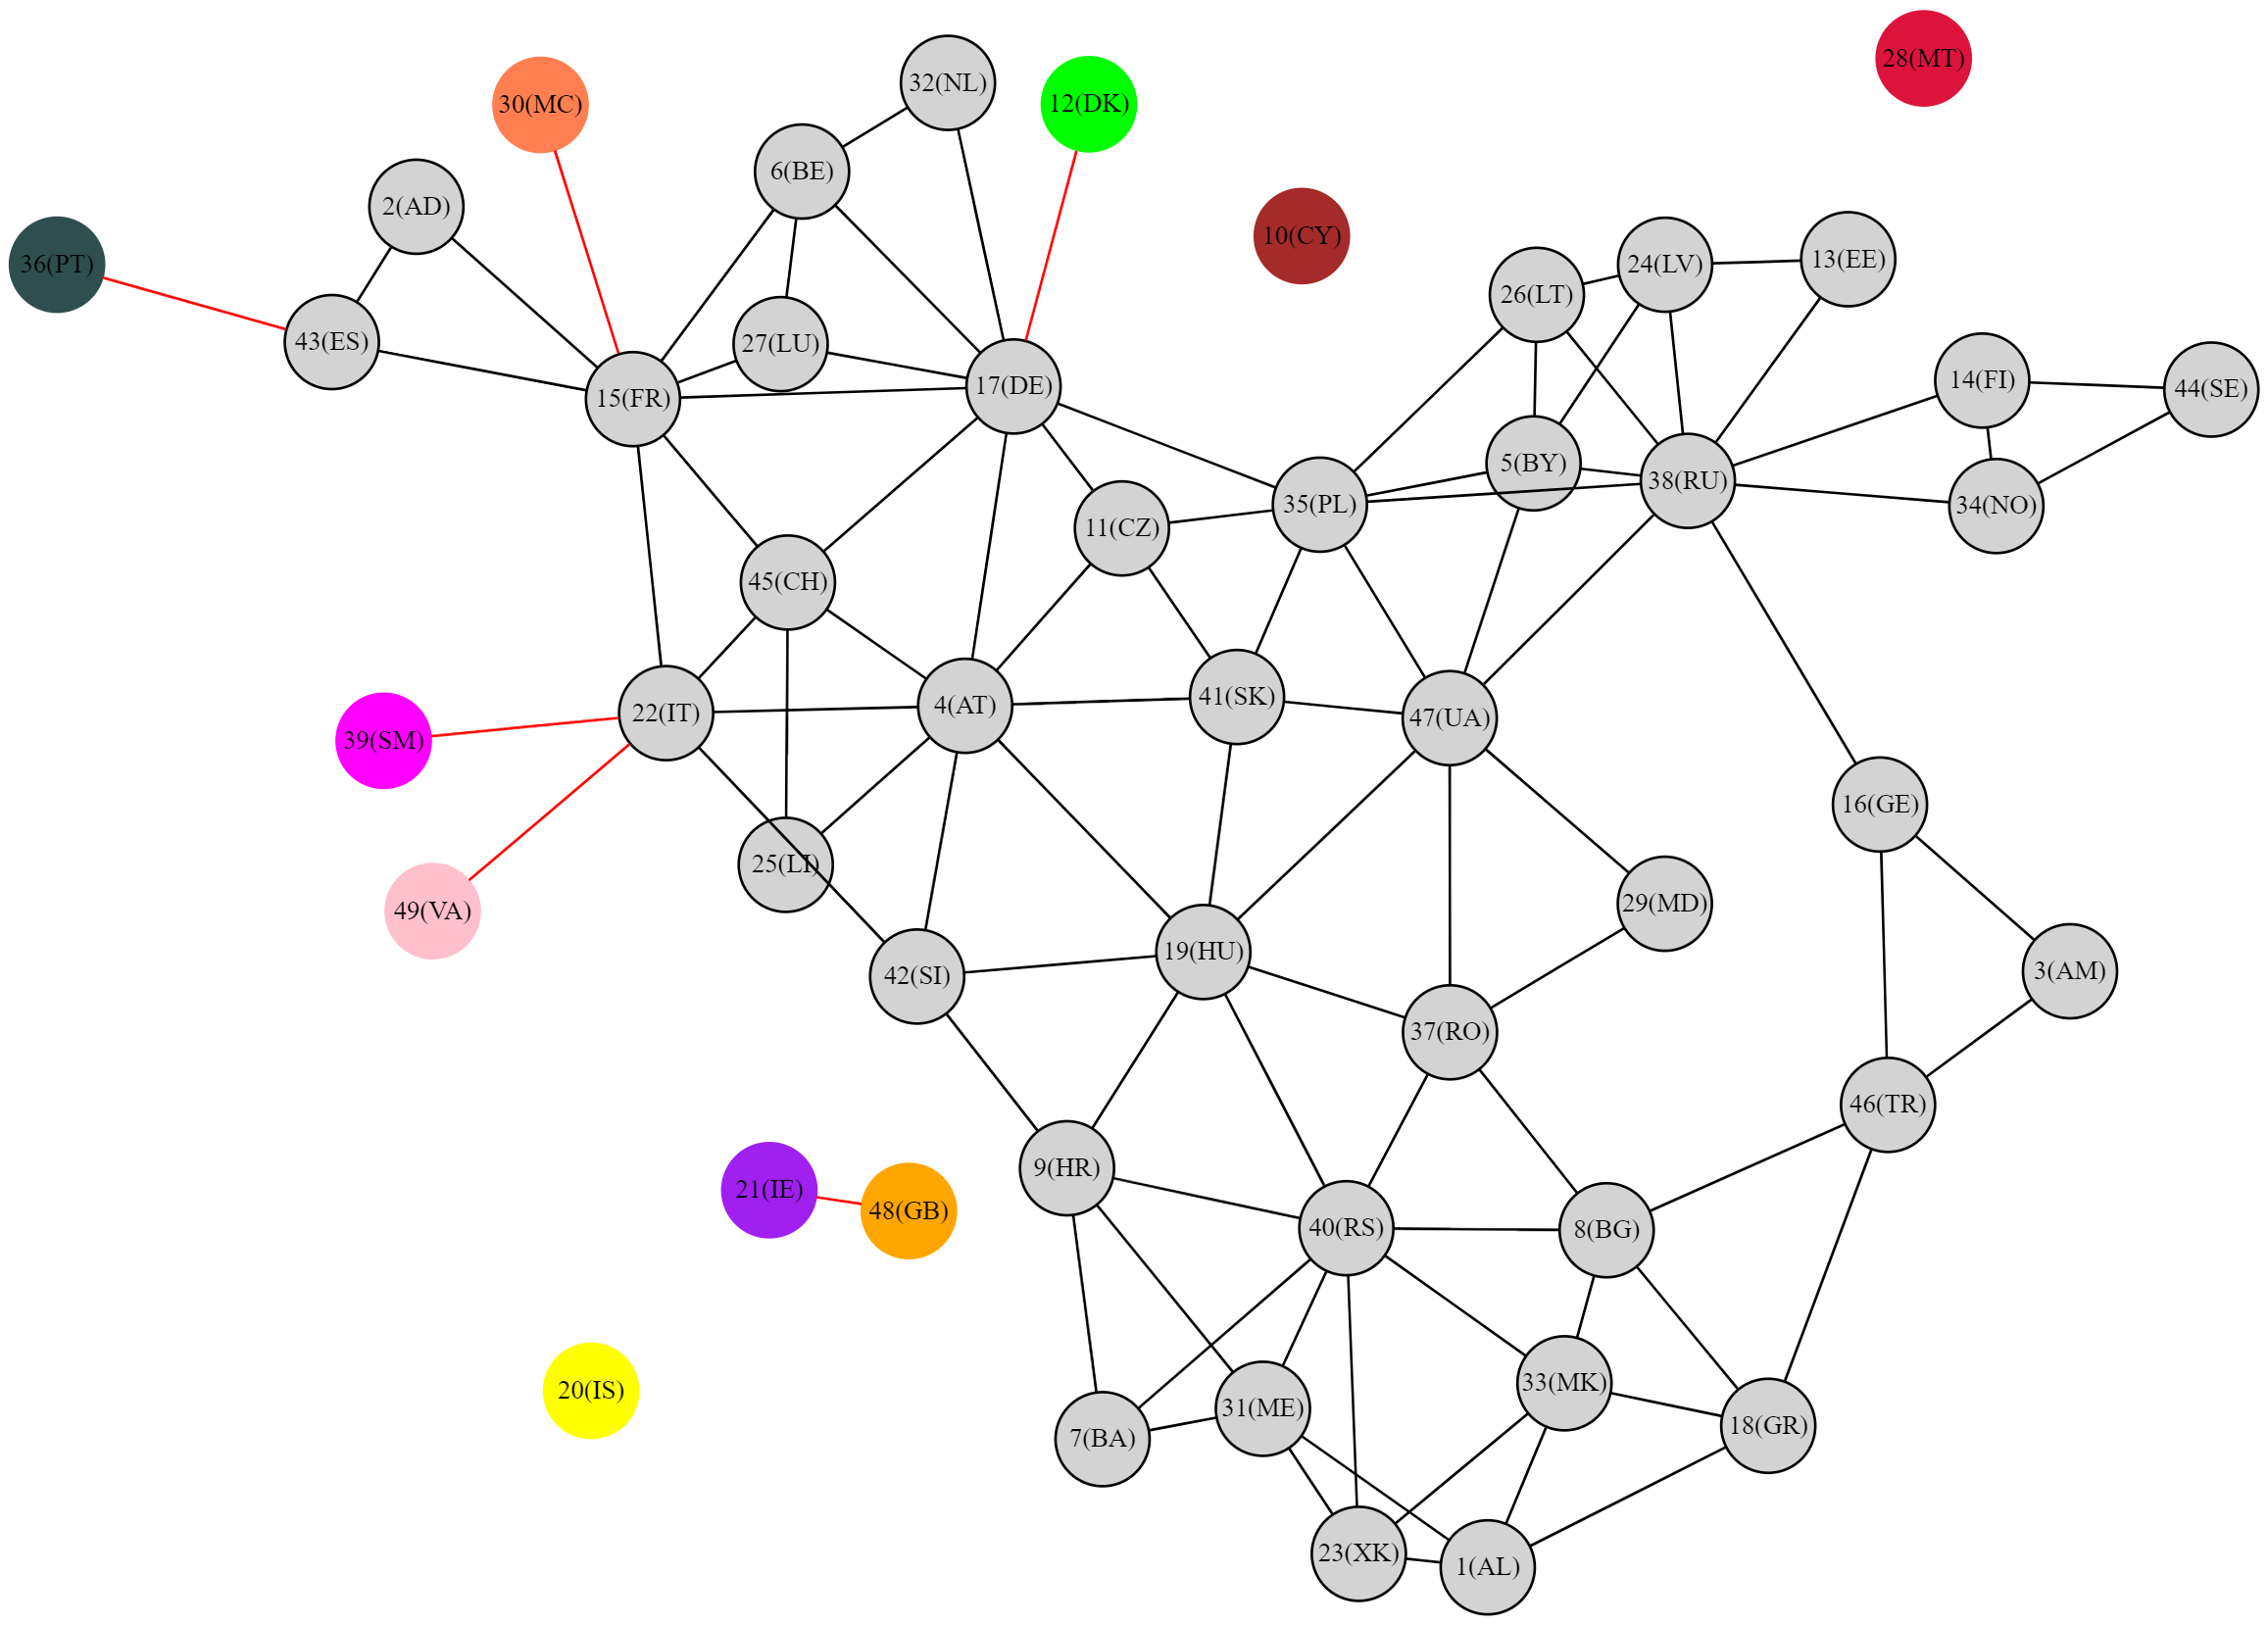
\includegraphics[width=1\textwidth]{2edge.png}
		\caption{Bridges are painted red, different 2-edge-connected components are painted differently (grey vertices are also in the component)}
	\end{figure}\newpage
	(n) Even though the codomain of {\footnotesize$\mathcal{W}$} is $\mathds{R}$, rounded geodesic distance in km was used (numbers are still real). Prim's algorithm was used.
	\begin{figure}[h]
		\centering
		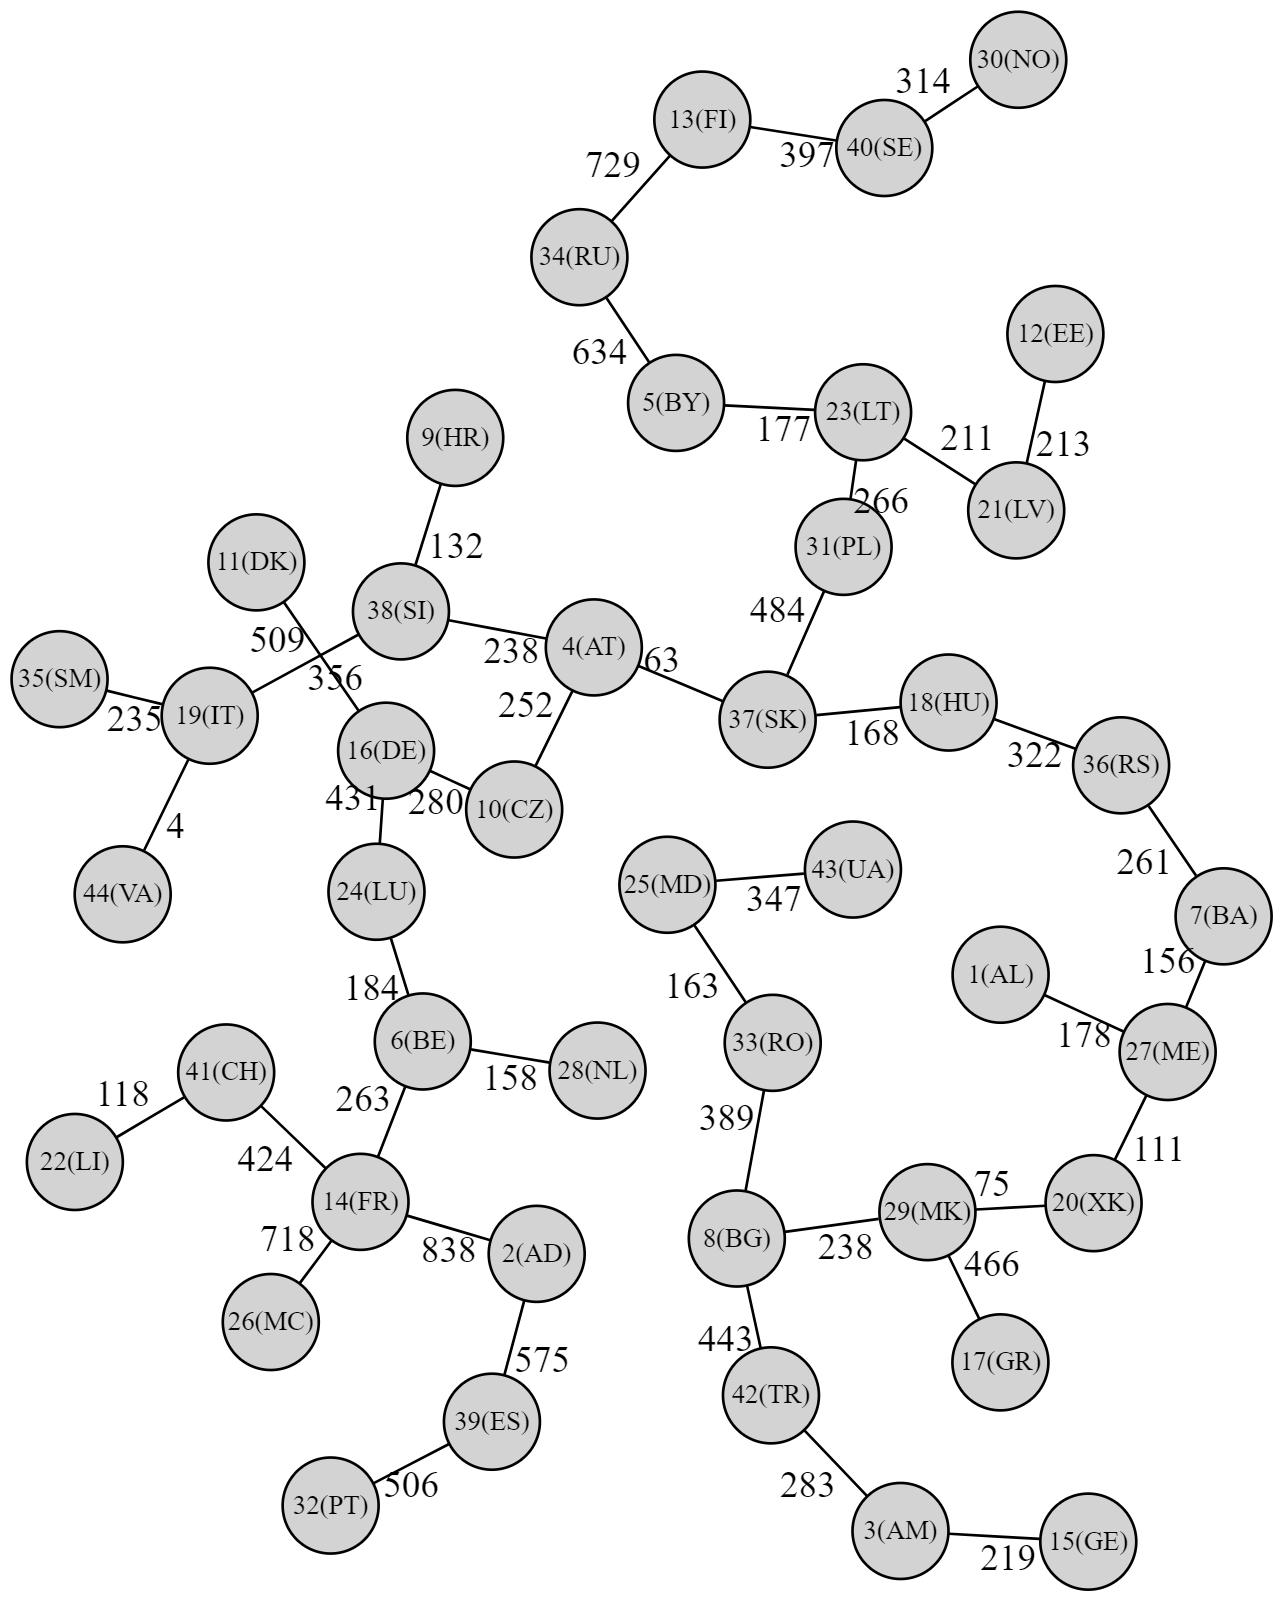
\includegraphics[width=0.8\textwidth]{tree.png}
		\caption{MST}
	\end{figure}\newpage
	(o) To find centroid, minimum of maximum branch weights of all vertices was calculated via C++. So the centroid is \{37(SK)\}.
	\begin{figure}[h]
		\centering
		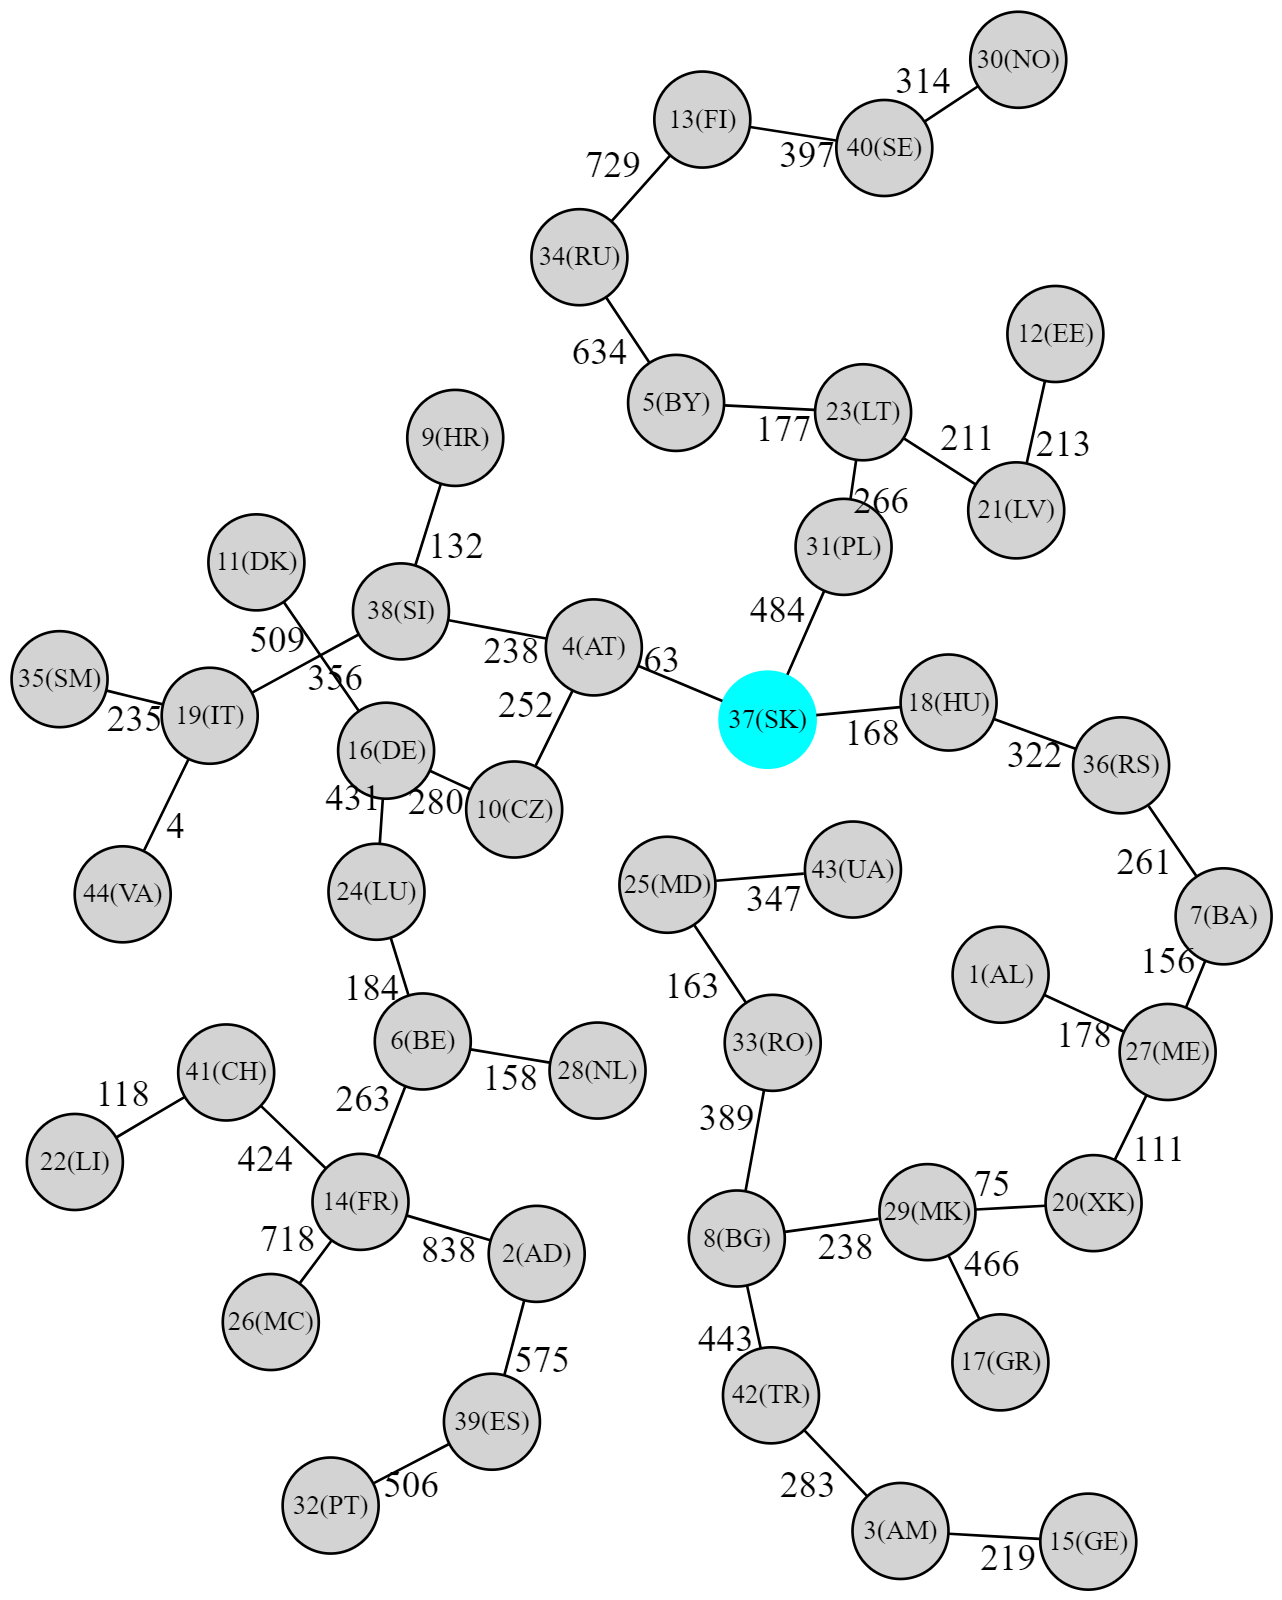
\includegraphics[width=0.8\textwidth]{centroid.png}
		\caption{Centroid is cyan}
	\end{figure}\newpage
	(p) Prufer code was calculated via C++. On each iteration we seek for the leafs -- vertices for which size of their adjacency list and erase them from their neighbour's list, adding neighbour to the code. The Prufer code (delimited by .) is :
	27.38.16.21.3.42.29.23.41.14.6.40.39.19.2.14.13.34.5.23.31.37.14.6.24.16.10.4.8.25.33.8.\\29.20.27.7.36.18.37.4.38.19 .
	\section*{Task 2}
	\textbf{Theorem 1.} $\forall x,y,z \in  V: \textmd{dist}(x,y)+ \textmd{dist}(y,z) \geq \textmd{dist}(x,z)$.\\
	Let $\textmd{dist}(x,z)$ be greater than $\textmd{dist}(x,y) + \textmd{dist}(y,z)$.\\
	$\exists $ shortest path $x \leadsto y = l_1 : |l_1| = \textmd{dist}(x,y)$;\\
	$\exists $ shortest path $y \leadsto z = l_2: |l_2| = \textmd{dist}(y,z)$.\\
	Then there is walk $l_3$ from $x$ to $z$, which consisits of $l_1$ and $l_2$, and its length is $|l_1| + |l_2|$. $|l_3| = \textmd{dist}(x,y) + \textmd{dist}(y,z)$, and as it can contain cycles, we can delete redundant edges from the walk to make the path $x \leadsto z$. Then $|x \leadsto z| \leq |l_3| = \textmd{dist}(x,y) + \textmd{dist}(y,z)$ and, as $\textmd{dist}(x,y) + \textmd{dist}(y,z) < \textmd{dist}(x,z)$, $|x \leadsto z| < \textmd{dist}(x,z)$. But $\textmd{dist}(x,z)$ is the length of the shortest path from $x$ to $z$ and we've found the path which is shorter than the shortest one. It's contradiction, so $\forall x,y,z \in  V: \textmd{dist}(x,y)+ \textmd{dist}(y,z) \geq \textmd{dist}(x,z)$.\\\\
	\textbf{Theorem 2.} A connected graph $G = \langle V, E \rangle$ is a tree (i.e. acyclic graph) \textit{iff} $|E| = |V| - 1$.\par
	$\Longrightarrow$:\\
	As $G$ is connected, there is a unique path between any two vertices of it (if there were 2 distinct paths, we would manage to take subpaths so that they would end and begin in the same vertices and would be internally vertex-disjoint -- in that case we would be able to form a cycle, but $G$ is acyclic). If we delete from $G$ any edge $e$, the unique path between its incident vertices will be lost, therefore $G$ will become disconnected. Hence, $\forall e \in E(G): G - e$ is disconnected.\\
	For $K_1$ (the only tree on 1 vertex): $0 = 1 - 1$ -- the theorem works.\\
	For $K_2$ (the only tree on 2 vertex): $1 = 2 - 1$ -- the theorem works.\\
	Assume that for any tree on $k < n$ vertices $|E| = k - 1$.\\
	Consider a tree on $n \geq 3$ vertices: we'll delete arbitrary edge to disconnect a tree, now connected components $G_1$ and $G_2$ are trees as well (if they had cycles, $G$ would have them too) and, as for both of them number of vertices is less than $n$, $|E_1| = |V_1| - 1$, $|E_2| = |V_2| - 1 \rightarrow |E_1| + |E_2| = |V_1| +|V_2|- 2$. As they're connected components of $G$ and only one edge of $G$ doesn't belong to any of them, $|V_1| +|V_2| = |V|$ and $|E_1| + |E_2| = |E| - 1$. So,
	$|E| - 1 = |V| - 2 \leftrightarrow |E| = |V| - 1$ for $G$. As we've chosen arbitrary tree of size $n$, every tree of size $n$ has $n - 1$ edges, and we can use all of them in next steps of induction.\par
	$\Longleftarrow$:\\
	Assume that connected graph $G$, which has at least one cycle, has $|V| - 1$ edges. We'll get a tree with the same number of vertices by deleting at least one edge to get rid of cycles. Since at least one edge was deleted number of edges in the tree on $|V|$ vertices is less than $|V| - 1$, which contradicts proven in  $\Longrightarrow$ paragraph, so $G$ shouldn't contain any cycles -- it should be a tree.\\\\\\
	\textbf{Theorem 3.} For any bipartite graph $G = (X,Y,E)$, there exists $X$-perfect matching (set of disjoint edges covering all vertices in $X$) \textit{iff} $|N(W)| \geq |W| $ for every $W \subseteq X$.\par
	$\Longrightarrow$:\\
	If there exists $X$-perfect matching, every vertex of $X$ has at least one neighbour in $Y$. If a vertex from $Y$ is matched to some vertex from $X$, there can't be matched edge from it to another vertex in $X$. Then every vertex in $X$ has unique matched neighbour, and $\forall W \subseteq X: |N(W)| \geq |W|$.\par 
	$\Longleftarrow$:\\
	Assume that $X$-perfect matching doesn't exist. Then we can take maximum matching $M$ -- at least one vertex $u$ from $X$ is unmatched. Consider all alternating paths (that use alternately edges which are in $M$ and which aren't), starting from $u$. Let $S$ be set of the vertices in such paths. Let $W = S \cap X$, $Z = S \cap Y$. then every vertex in $Z$ is matched by $M$ to a vertex in $W$ (if some vertex $z \in Z$ wasn't in $M$, we could make matching of size $|M| + 1$ by adding to M edges from path, which aren't in $M$, and deleting from matching those edges, which are in $M$ as the endpoints of the path would be unmatched). The size of $W$ is at least $|Z| + 1$ as there are $|Z|$ pairwise non-adjacent edges between vertices of $Z$ and $W$, and vertex $u$ isn't incident to any of them. So, $|W| > |Z|$.\\
	$\forall v \in W$: every neighbour $z$ of $v$ is in $Z$. If edge $vz$ is unmatched, we can add it to alternating path that ends with matched edge to $v$. If $vz$ is matched, it's either used in path $u \leadsto v$ or can be added to it as all other incident to $v$ edges are unmatched. Therefore, $Z = N(W)$, $|W| > N(W)$. This is a contradiction, so $X$-perfect matching exists.\\\\
	\textbf{Theorem 4.} For any graph $G$: $\varkappa(G) \leq \lambda(G) \leq \delta(G)$.\\
	If $G$ is disconnected or trivial, $\varkappa(G) = \lambda(G) = \delta(G) = 0$. For $K_2$: $1 \leq 1 \leq 1$. \par
	$\lambda(G) \leq \delta(G)$:\\
	Assume $\lambda(G) > \delta(G)$. then removing $\delta(G)$ edges shouldn't disconnect the graph. We'll choose the vertex which degree is equal to $\delta(G)$ and delete all its incident edges. As number of its incident edges is $\delta(G)$, the graph should remain connected but it doesn't as this vertex now hasn't any adjacent vertices. This is contradiction, so $\lambda(G) \leq \delta(G)$.\par 
	$\varkappa(G) \leq \lambda(G)$:\\
	If $G$ has a bridge, $\lambda(G) = 1$ and deleting one of its endpoints makes $G$ disconnected (if connected $G$ is not $K_2$, at least one endpoint has degree more than 1 and its deleting disconnects graph), so $\varkappa(G) = 1 \leq\ 1$. If $\lambda(G) \geq 2$, we can delete $\lambda(G) - 1$ edge -- graph is still connected and at least one its edge is a bridge. For each of deleted edge we can choose vertex incident to it (this vertex shouldn't be incident to our bridge) and delete it. This action deletes the same edges that we've deleted before and can delete even more, but doesn't delete bridge endpoints. If $G$ is now disconnected, $\varkappa(G) < \lambda(G)$, else we can delete one of bridge endpoints and $\varkappa(G) = \lambda(G)$. So $\varkappa(G) \leq \lambda(G)$.\\\\
	\textbf{Theorem 5.} For a connected graph $G = \langle V, E\rangle$: if $\delta(G) \geq\lfloor|V|/2\rfloor$, then $\lambda(G) = \delta(G)$.\\
	By deleting $\lambda(G)$ edges, we split $G$ into several connected components. Let $C$ be the smallest one (by size in vertices), $|C| = k$. Then $1 \leq k \leq \lfloor |V|/2 \rfloor \leq \delta(G)$ (else it wouldn't be smallest). Consider vertex $v \in C$: it's incident (in $G$) to at least $\delta(G)$ edges. At most $k - 1$ of them are incident to other vertices from $C$, so at least $\delta(G) - (k - 1)$ edges connect $v$ and vertices from $V \backslash C$. So there are at least $k(\delta(G) - (k - 1))$ edges between this component and other vertices. Therefore, $\lambda(G)$ is greater than minimum value of this expression (enumerating through all $k$). As this function is quadratic and its maximum is on $\frac{\delta(G) + 1}{2}$, it's minimum value is on $1$ (the same value is on $\delta(G)$ which is at least $k$'s upper bound), $\lambda(G) \geq 1 * (\delta(G) - 1 + 1) = \delta(G)$. But due to the Whitney's theorem $\lambda(G) \leq \delta(G)$, so $\lambda(G) = \delta(G)$.\newpage
	\textbf{Theorem 6.} For any pair of non-adjacent vertices $u$ and $v$ in an undirected graph, the size of the minimum vertex cut is equal to the maximum number of pairwise internally vertex-disjoint paths from $u$ to $v$.\par
	The theorem works for null graph and $K_1$ as there aren't any pairs of non-adjacent vertices. If $u$ and $v$ are in different components, their vertex cut size is 0 and there are no paths between them. So we're considering vertices from one component. If minimum vertex cut size $k$ is 1, there is only one internally vertex-disjoint path from $u$ to $v$. So, consider $k \geq 2$.\\
	Assume that for every graph of less size, the theorem works. Then there are 3 cases for graph of size $m$:\par
	1) Minimum vertex cut $C$ contains a vertex $c$ that is adjacent to both $u$ and $v$. Then $C \backslash c$ is miminum in graph $G - c$, which size is less than size of $G$, hence the theorem is true for it, there are $k - 1$ disjoint paths. Together with $u-c-v$ there are $k$ such paths in $G$.\par
	2) All vertices in every minimum vertex cut $C$ are adjacent to only $u$ or only $v$. Then $\textmd{dist}(u,v) \geq 3$ (as $c$ would be adjacent to both). Let this shortest path be $u - x - y -...-v$, let $xy$ be $e$. Then every $C$ in $G - e$ contains at least $k - 1$ vertices. Let some minimum cut of size $k - 1$ be $Z = {z_1,z_2,...,z_{k-1}}$. Then $Z \cup {x}$ is a cut in $G$ and therefore a minimum cut in $G$. Since $x$ is adjacent to only $u$, all $z_i$ are adjacent to only $u$ as well. $Z \cup {y}$ is also minimum cut in $G$ and all $z_i$ are adjacent to only $u$, $y$ is also adjacent to $u$. But then the path is not the shortest. This is contradiction, so cut $C$ in $G - e$ contains at least $k$ vertices.  Since the
	size of $G - e$ is less than $m$, it follows that there are $k$ internally disjoint $u-v$ paths in $G - e$ and in $G$ as well.\par 
	3) 	There is some cut $C$ that no vertex in it is adjacent to both vertices and $C$ contains at least one vertex not adjacent to $u$ and at least one vertex not adjacent to $v$. Let $C = {c_1,c_2,..,c_k}$. Let $G_u$ be the subgraph of $G$ consisting of all $u - c_i$ paths in $G$ in which $c_i$ is the only vertex of the
	path belonging to $C$. Let $G'_u$ be the graph constructed from $G_u$ by adding a
	new vertex $v'$ and joining it to each vertex $c_i$. The graphs $G_v$ and $G_v'$ are defined similarly. Since $C$ contains a vertex that is not adjacent to $u$ and a vertex that is not
	adjacent to $v$, the sizes of both $G'_u$ and $G'_v$ are less than $m$. So $G'_u$ contains $k$ $u-v'$ paths $A_i$. Also, $G'_v$ contains $k$ $u'-v$ paths $B_i$. Let $A_i' = u - c_i'$ subpath of $A_i$ and $B_i' = v - c_i'$ subpath of $B_i$. The $k$ paths constructed from $A_i'$ and $B_i'$ for each $i$ are internally disjoint $u - v$ paths in $G$.\newpage
	\textbf{Theorem 7.} Every block of a block graph is a clique.\\
	$K_2$ is complete, there is only $K_3$ block on 3 vertices.
	For blocks of size $\geq 4$: let block graph be $H$, original graph $G$. Consider $B$ -- block of $H$. 
	Let it be not complete. then there is a pair of non-adjacent vertices and, as they're in block they belong to some cycle which length is at least 4(they're non-adjacent). Then any vertices in two blocks (to which these 2 vertices correspond) in $G$ are connected through different blocks from cycle and union of blocks from cycle hasn't any cut vertices, which means that this union is a part of some block. But each block in it is already maximal -- contradiction. So every $B$ is clique.
\end{document}
